\documentclass[compress,t,usenames,xcolor=dvipsnames]{beamer}

\usepackage{beamerthemeTUM_blue}
\setbeamersize{text margin left=1cm}

\usepackage[english]{babel}
\usepackage[utf8]{inputenc}

% hide notes | show notes | show notes on second screen=<location> | show only notes
\setbeameroption{hide notes}
\beamertemplatenavigationsymbolsempty %hide beamer navigation symbols

% Color Definitions
\definecolor{SourceColor}{RGB}{85,168,104}
\definecolor{TargetColor}{RGB}{221,132,82}
\definecolor{TargetChangerColor}{RGB}{255,153,0}
\definecolor{AbsorbingAreaColor}{RGB}{196,78,82}
\definecolor{ObstacleColor}{RGB}{179,179,179}
\definecolor{StairColor}{RGB}{129,114,178}
\definecolor{MeasurementAreaColor}{RGB}{255,0,0}
\definecolor{AgentColor}{RGB}{76,114,202}
\definecolor{AgentIdColor}{RGB}{255,127,0}

\usepackage{lmodern}
% Perception layer
\colorlet{PerceptionColor}{RoyalPurple}
\colorlet{CognitionColor}{RedViolet}
\colorlet{LocomotionColor}{Gray}

% A list which should be used in tabular environments
\usepackage[export]{adjustbox}
\usepackage{amsmath, amssymb, amsfonts, amsthm}
\usepackage{appendixnumberbeamer}
\usepackage[
    sorting=nyt,      % nyt | nty | nyt | nyvt | anyt | ynt | ydnt | none | debug
    style=authoryear, % numeric | alphabetic | authoryear | authortitle | verbose | draft | debug
    uniquename=false, % true, false , init, full, allinit, allfull, mininit, minfull
]{biblatex}
\addbibresource{./Literatur/Literature.bib}
\usepackage{csquotes}
\usepackage{float}
\usepackage{fontawesome}
\usepackage{graphicx}
\graphicspath{{./Figures/}{./Videos}}
\DeclareGraphicsExtensions{.pdf,.png,.jpg}
\usepackage{hyperref}
\usepackage{pgfkeys}
\usepackage[per-mode=symbol,separate-uncertainty]{siunitx}
\usepackage{subcaption}
% Remove prefix like "Figure: " from "figure" and "subfigure" environment.
\captionsetup[figure]{labelformat=empty}
\captionsetup[subfigure]{labelformat=empty}
\usepackage{tikz}
\usepackage{url}
\usepackage{multirow}

\usepackage{listings} 
\lstset{
    backgroundcolor=\color{white},
    basicstyle=\ttfamily\tiny,
    breakatwhitespace=false,
    breaklines=true,
    captionpos=b,
    commentstyle=\color{mygreen},
    % deletekeywords={},
    escapeinside={\%}{\%},
    escapechar=\%,
    extendedchars=true,
    firstnumber=1,
    frame=single,
    keepspaces=true,
    keywordstyle=\color{blue},
    language=Java,
    morekeywords={*,eventController,cognitionLayer},
    % numbers=left,
    numbersep=5pt,
    numberstyle=\tiny\color{mygray},
    rulecolor=\color{black},
    showspaces=false,
    showstringspaces=false,
    showtabs=false,
    stepnumber=1,
    stringstyle=\color{mymauve},
    tabsize=2,
    title=\lstname
}
\resetcounteronoverlays{lstlisting}

\usepackage{tabularx}
% M centers cells vertically and the extra "\centering" centers cell content horizontally
\newcolumntype{M}[1]{>{\centering\arraybackslash}m{#1}}
% Use smaller space for itemizes environemt inside tabulars
\newenvironment{itemizetab}{\begin{itemize}\setlength\itemsep{1mm}\setlength{\baselineskip}{1mm}}{\end{itemize}}

%-------------------------------------------------------------------------------
% User-Defined Commands
%-------------------------------------------------------------------------------
\newcommand{\ie}{that is} % this is better, when you read aloud, also better English
\newcommand{\Ie}{That is} % this is better, when you read aloud, also better English
\newcommand{\eg}{e.\,g.}
\newcommand{\Eg}{E.\,g.}
\newcommand{\code}[1]{\texttt{#1}}
\newcommand{\program}[1]{\texttt{#1}}
\newcommand{\q}[1]{\textit{\enquote{#1}}}

\newcommand{\cvtag}[1]{%
    \tikz[baseline]\node[anchor=base,draw=black!30,rounded corners,inner xsep=0.5ex,inner ysep =0.5ex,text depth=.25ex]{#1};
}
% Cite pages or page ranges (and use normal or non-breaking spaces)
\newcommand{\p}[1]{p.\,#1}
% When citing a source, name source type (e.g. image) and the source, e.g. "image: Picasso 1900"
\newcommand{\src}[2]{#1: #2}
\newcommand{\srcimg}[1]{\src{image}{#1}}
\newcommand{\srcphoto}[1]{\src{photo}{#1}}
\newcommand{\srclst}[1]{\src{listing}{#1}}
\newcommand{\srctab}[1]{\src{table}{#1}}
\newcommand{\srcinsp}[1]{\src{own graphic but inspired by}{#1}}
\newcommand{\legend}[1]{\textcolor{#1}{\(\blacksquare\)}}

\newcommand{\todo}[1]{\textcolor{red}{TODO #1}}
\newcommand{\ResearchQuestion}{How can changes in human behavior be operationalized for simulations?}
\newcommand{\researchQuestion}{how can changes in human behavior be operationalized for simulations?}

\providecommand{\norm}[1]{\lVert#1\rVert}
\DeclareMathOperator*{\argmax}{arg\,max}

\newcommand{\twocolcaption}{
    \vspace{\baselineskip}
    \begin{columns}
        \begin{column}{0.5\linewidth}
            \centering
            Operationalization
        \end{column}
        \begin{column}{0.5\linewidth}
            \centering
            Simulator
        \end{column}
    \end{columns}
}

% The "\vlink" command to show a preview image of a video file with a "play button" overlay using TikZ
% Before compiling, call "./create_video_previews.sh"!
\pgfkeys{
    /vlink/.is family, /vlink, % Create key family to avoid name clashes
    default/.style =  {
        color=white,
        opacity=0.60,
        playbuttonscale=0.5,
        width=\textwidth
    },
    color/.estore in = \vlinkColor,
    opacity/.estore in = \vlinkOpacity,
    playbuttonscale/.estore in = \vlinkPlayButtonScale,
    width/.estore in = \vlinkWidth
}
\newcommand\vlink[2][]{%
    \pgfkeys{/vlink, default, #1}% Call "pgfkeys" with family, default values and optional first command parameter
    \tikz{
        \node (previewimage)
        {\href{run:#2}{\includegraphics[width=\vlinkWidth]{{{#2.preview}}}}};
        \node [align=center,color=\vlinkColor,opacity=\vlinkOpacity,text width=\vlinkWidth] at
        (previewimage.center){\fontsize{\vlinkPlayButtonScale\dimexpr\vlinkWidth\relax}{\vlinkWidth}\selectfont\faPlayCircleO};
    }
}

\newenvironment{changemargin}[2]{% 
  \begin{list}{}{%
    \setlength{\topsep}{0pt}%
    \setlength{\leftmargin}{#1}%
    \setlength{\rightmargin}{#2}%
    \setlength{\listparindent}{\parindent}%
    \setlength{\itemindent}{\parindent}%
    \setlength{\parsep}{\parskip}%
  }%
  \item[]}{\end{list}}

\newcommand{\logoheight}{0.6\baselineskip}
\newcommand{\tocimage}[1]{\includegraphics[width=0.5\textwidth]{Introduction/ResearchQuestion/ResearchQuestionAndResearchMethods-Highlighted-#1}}
\newcommand{\myshow}{1.0}
\newcommand{\myhide}{0.2}
% Create a short TOC for each part of the talk where inactive parts ar gayed out
% Usage: \tocprogress[\tocimage{01}]{\myshow}{\myhide}{\myhide}
\newcommand{\tocprogress}[4][]{
\setbeamertemplate{footline}{} % remove footer
\begin{frame}[c,noframenumbering]{Outline}
    \begin{enumerate}
        \pgfsetfillopacity{\myhide}
        \item \hyperlink{sec:ResearchQuestion}{Motivation and research question}
        \item  \hyperlink{sec:ModelingAndMyExperiment}{Highlights}
        \begin{itemize}
            \setlength\itemsep{0.5\baselineskip}
            \pgfsetfillopacity{#2}
            \item \hyperlink{sec:ModelingAndMyExperiment}{Modeling: Approaches and my experiment}
            \pgfsetfillopacity{#3}
            \item \hyperlink{sec:Implementation}{Implementation: A reusable psychology layer}
            \pgfsetfillopacity{#4}
            \item \hyperlink{sec:Validation}{Validation: 2nd --- perceived threat}
        \end{itemize}
    \end{enumerate}
    \begin{flushright}
        #1
    \end{flushright}
\end{frame}
\setbeamertemplate{footline}[infolines theme]
}

\title{How to simulate crowds and behavioral changes}
\subtitle{In a nutshell}
\author{Benedikt Kleinmeier} 
\institute{}
\date{\today}
\titlegraphic{Template/Vadere-Bottleneck-Framed}
% \logo{
\includegraphics[height=0.4cm]{Figures/Template/TUM_Logo_RGB}}

% Show table of contents before entering a section
% \AtBeginSection[]{
% \setbeamertemplate{footline}{} % remove footer for the last slide
% \begin{frame}[c]{Outline}
%     \setbeamertemplate{sections/subsections in toc}[ball]
%     \tableofcontents[currentsection,currentsubsection]
% \end{frame}
% \setbeamertemplate{footline}[infolines theme]
% }

% Count from the actual content i.e. after the title page
\addtocounter{framenumber}{-1}

% Goal: The audience should get familiar with pedestrian dynamics, state-of-art modeling approaches and my work and contributions
\begin{document}

\begin{frame}[plain]
\titlepage

\note[item]{Hi and welcome everybody to my talk about \enquote{\inserttitle}.}
\note[item]{I am Benedikt and I am working in the pedestrian dynamics research group at Munich's University of Applied Sciences.}
\end{frame}

\setbeamertemplate{footline}{} % remove footer for the last slide
\begin{frame}[c]{Outline}
    \setbeamertemplate{sections/subsections in toc}[ball]
    \tableofcontents[hideallsubsections]
\end{frame}
\setbeamertemplate{footline}[infolines theme]

\section{About me}

\begin{frame}{About me}
    \begin{block}{\alert{I am} a computer scientist}
        \begin{itemize}
            \item Firmware development for different MCUs
            \item Application development
        \end{itemize}
        \(\Rightarrow\) I.e., a strong focus on software engineering, test-driven development and CI/CD.
    \end{block}
    \begin{block}{\alert{I am not} an electrical engineer / UX designer}
        \begin{itemize}
            \item No deep hardware knowledge!
        \end{itemize}
        \(\Rightarrow\) I am not an expert, but I am very interested in hardware and data visualization.
        % But, since my work at Infineon I am very interested in understanding what's going on on physical level.
    \end{block}
\end{frame}

\begin{frame}{Curriculum}

    \begin{itemize}
    \uncover<1->{
        \item 2008--2014: Computer science at Hochschule München \hfill 
\includegraphics[height=\logoheight]{Template/HM_Logo_rot_RGB_Cut}
        \begin{itemize}
            \item BA thesis: Firmware to get data from a pressure sensor and a GUI to visualize this data: \cvtag{C} \cvtag{C\#} \cvtag{.NET}
            \item MA thesis: Linux driver to acquire data from a GPS sensor: \cvtag{C} \cvtag{C++} \cvtag{Real-Time Linux}
        \end{itemize}
    }
    \uncover<2->{
        \item 2015--2017: Firmware developer at Infineon \hfill 
\includegraphics[height=\logoheight]{Template/Infineon-Logo}
        \begin{itemize}
            \item Bootstrap loader (ARM-based MCUs): \cvtag{C}
            \item Firmware/Startup software (Aurix 2G): \cvtag{C} \cvtag{Python} \cvtag{TDD} \cvtag{CI/CD}
        \end{itemize}
    }
    \uncover<3->{
        \item Since 12/2017: PhD at HM and TUM \hfill 
\includegraphics[height=\logoheight]{Template/HM_Logo_rot_RGB_Cut} \& 
\includegraphics[height=\logoheight]{Template/TUM_Logo_RGB}
        \begin{itemize}
            \item Modeling and simulation of behavioral changes
            \item Using open source simulator Vadere (\url{http://www.vadere.org/})
            \item Pedestrian dynamics research group (Prof. Dr. Köster, Hochschule München) \\ \cvtag{Java} \cvtag{Python} \cvtag{matplotlib} \cvtag{TDD} \cvtag{CI/CD}
        \end{itemize}
    }
    \end{itemize}
 
\end{frame}

\section{Crowd simulations}

\subsection{Motivation}

\begin{frame}{Motivation}
    \begin{block}{Why do we need pedestrian dynamics?}
        \vspace{-2mm}
        \begin{figure}
            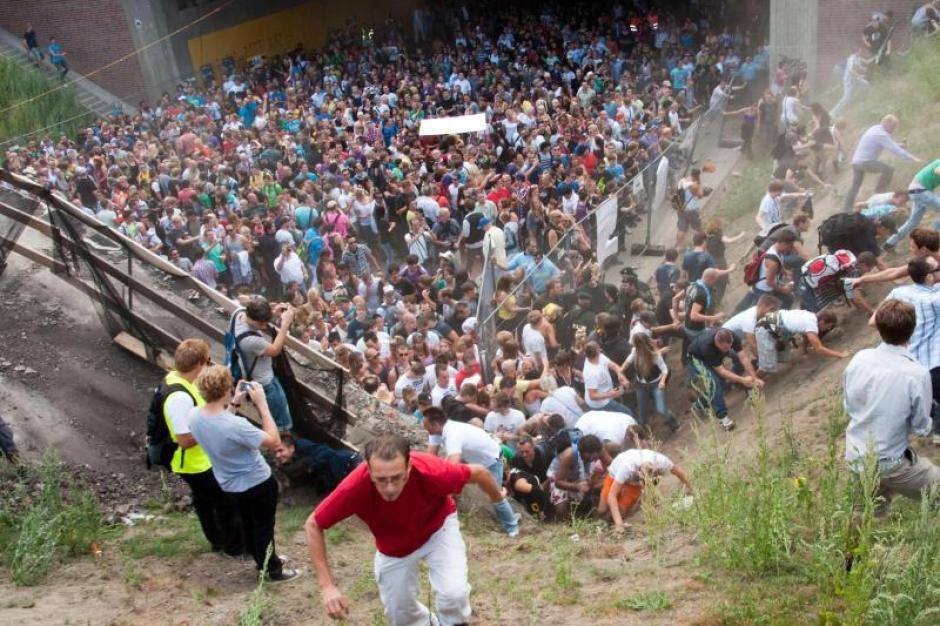
\includegraphics[width=0.7\textwidth]{Introduction/LoveParade-2010-Stampede}\\[-2mm]
            \caption{Stampede at Love Parade, Duisburg, 2010, \srcphoto{\cite{wiffers-2010}}}
        \end{figure}
        \vspace{-6mm}
        \alert{Goal:} Reduce risks for life and limb wherever crowds gather by getting insights into pedestrian streams with simulations
    \end{block}
    
    \note[item]{There have been numerous crowd disaster with injureds and casualties.}
    \note[item]{The research field of pedestrian dynamics tries to better understand crowd behavior to avoid such disasters.}
    \note[item]{On the empirical side, pedestrian dynamics researchers carry out experiments and where this is not possible simulations are carried out.}
    \note[item]{The goal is to reduce risks for life and limb wherever crowds gather.}
\end{frame}

\begin{frame}{How to simulate crowds}
    
    \begin{block}{Two main problems:}
    \begin{columns}
        \column{0.5\textwidth}
        \centering
        1. Navigation and wayfinding (solved \(\rightarrow\) next slide) \\[4mm]
        \includegraphics[width=0.9\linewidth]{kleinmeier-2019/Simulations/BasicComponents} \\
        {\tiny \legend{SourceColor}: source, \legend{TargetColor}: target, \legend{ObstacleColor}: obstacles, \legend{AgentColor}: agents\par}
        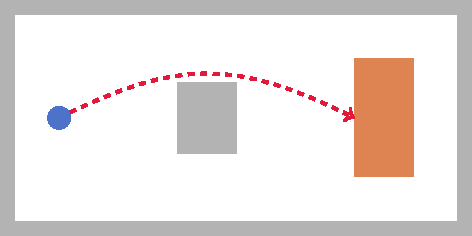
\includegraphics[width=0.9\linewidth]{Figures/kleinmeier-2019/Simulations/FloorField-GeodesicDistance}
        \column{0.5\textwidth}
        \centering
        2. Behavioral changes (unresolved \(\rightarrow\) my PhD) \\[3mm] % Mention my three pillars: experiment, research project and research stay
        \vlink[color=white,width=\textwidth]{./Videos/Validation-UseCase1-CooperativeCognitionModel-Disabled.mp4}
    \end{columns}
    \end{block}
    
\end{frame}

% I based my implementation on an existing locomotion layer
\subsection{Current state: Navigation and wayfinding}

\begin{frame}{Navigation and wayfinding: Our approach}
    \begin{columns}[T]
        \column{0.5\textwidth}
        \begin{minipage}[c][0.4\textheight][t]{\textwidth}
            \alert<1-2>{1. A floor field based on the eikonal equation:}\\[2mm]
            \(| \nabla u(x)| = \frac 1 {f(x)}, x \in \mathbb{R}^2 \)
            \begin{itemize}
                \item Solution \(u(x)\): encodes minimal distance from \(x\) to target curvature \(\partial \Omega\)
                \item Given: speed \(f(x)\)
                \item Fast marching method (finite differences)
            \end{itemize}
            \vspace{-1mm}
            \centering
            \only<1>{\includegraphics[width=0.725\textwidth]{PedestrianStreamSimulations/Microscopic/FloorField-Plot/ContourPlot-Corridor10x6m-RedBluColorMap-WithAgents}}
            \only<2->{\includegraphics[width=0.725\textwidth]{PedestrianStreamSimulations/Microscopic/FloorField-Plot/Vadere-EikonalEquation-Discretization}}
        \end{minipage}
        \column{0.5\textwidth}
        \begin{minipage}[c][0.4\textheight][t]{\textwidth}
            \alert<3->{2. An optimization for each agent in each simulation step (goal: reduce travel time)}
            \visible<3->{
                \begin{center}
                    \includegraphics[width=0.725\textwidth]{PedestrianStreamSimulations/Microscopic/FloorField-Plot/ContourPlot-Corridor10x6m-RedBluColorMap-WithAgentsAndSearchRadius}
                \end{center}
            }
        \end{minipage}
    \end{columns}
\end{frame}

\begin{frame}[c]{A crowd simulator}
    
    \begin{block}{Bird's eye view onto a simulator:}
        \lstinputlisting[caption={},label={lst:SimulationLoopVadere},language=Java]{Listings/Simulation-Loop.java}
    \end{block}
    
    \note[item]{Therefore, I visited the social psychology professor John Drury to dig deeper into crowds and crowd behavior.}
    \note[item]{By visiting his lectures, I was able to break down the process of behavioral changes into steps which are easy to implement.}
    \note[item]{Before going on, it is useful to conceptionally understand a crowd simulation tool.}
    \note[item]{But, this also holds true for any other simulation tool.}
    \note[item]{A crowd simulator is simple loop, in which the agent positions are adapted continuously.}
    \note[item]{Then, the simulation time is incremented.}
    
\end{frame}

\subsection{My work: Behavioral changes}

\begin{frame}[c]{Psychology layer: Overview}
    
    \begin{columns}
        \begin{column}[c]{0.5\linewidth}
            \begin{figure}
                \centering
                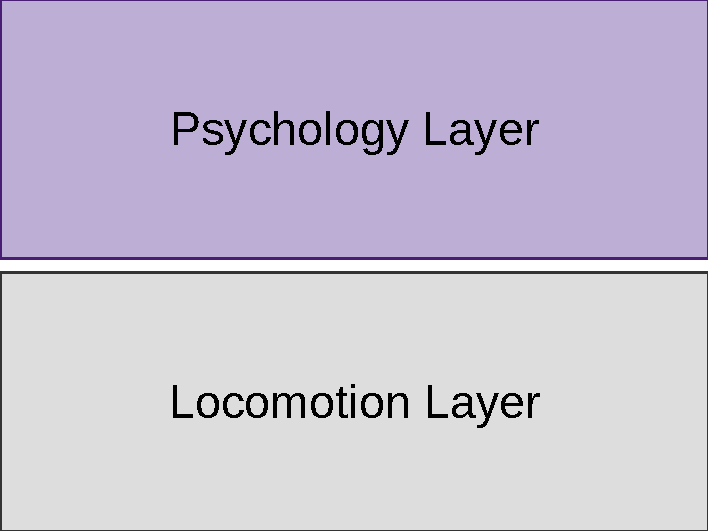
\includegraphics[width=\linewidth]{VaderePsychologyLayer/StepByStep/Vadere-PsychologyLayerSimple}
            \end{figure}
        \end{column}
        \begin{column}[c]{0.5\linewidth}
            \begin{figure}
                \centering
                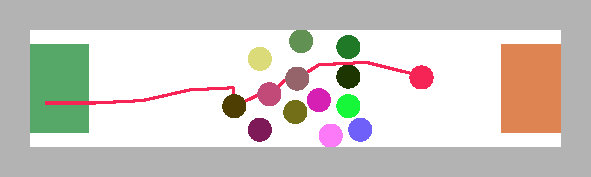
\includegraphics[width=\linewidth]{VaderePsychologyLayer/DisabledVsEnabled/CooperativeCognitionModel-PsychEnabled}
                \newline
                {\footnotesize With psychology \href{run:./Videos/Validation-UseCase1-CooperativeCognitionModel-Enabled.mp4}{\faPlayCircleO}}
                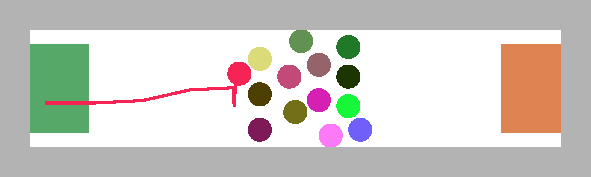
\includegraphics[width=\linewidth]{VaderePsychologyLayer/DisabledVsEnabled/CooperativeCognitionModel-PsychDisabled}
                \newline
                {\footnotesize Without psychology \href{run:./Videos/Validation-UseCase1-CooperativeCognitionModel-Disabled.mp4}{\faPlayCircleO}}
            \end{figure}
        \end{column}
    \end{columns}
    \twocolcaption{}
    
    \note[item]{I based by findings on existing microscopic locomotion strategies which is visualized as gray box on the left-hand side.}
    \note[item]{On top of that, I built an optional psychology layer which allows agents to change their behavior.}
    \note[item]{On the left-hand side, you see the conceptional and reusable aspects and on the right-hand side you see how I implemented this concept in the Vadere crowd simulator and how they can be used from a user's perspective.}
\end{frame}

\begin{frame}{Psychology layer: Result}
    \begin{block}{Bird's eye view onto a simulator:}
        \begin{columns}[T]
            \column{0.5\textwidth}
            \lstinputlisting[caption={},label={lst:SimulationLoopVadere},language=Java]{Listings/Simulation-Loop.java}
            \column{0.5\textwidth}
            \lstinputlisting[caption={},label={lst:SimulationLoopVadere},language=Java]{Listings/Simulation-LoopWithOptionalPerceptionLayer-Highlighted.java}
        \end{columns}
    \end{block}
    \begin{itemize}
        \item A minimally invasive psychology layer
        \item that can easily be integrated in other crowd simulators
    \end{itemize}
    
    \note[item]{These three aspects represent a generic approach to allow behavioral changes for a wide range of scenarios and can be reused also in other simulators.}
    \note[item]{If you compare the old simulation loop, you will see that...}
    \note[item]{...my psychology layer is minimally invasive}
    \note[item]{...and can easily be integrated in other crowd simulators}
    \note[item]{This was one of my primary goals to be beneficial fro the whole research community.}
    
\end{frame}

\begin{frame}[c]{Psychology layer: Optional}
    
    \begin{columns}
        \begin{column}[c]{0.5\linewidth}
            \begin{figure}
                \centering
                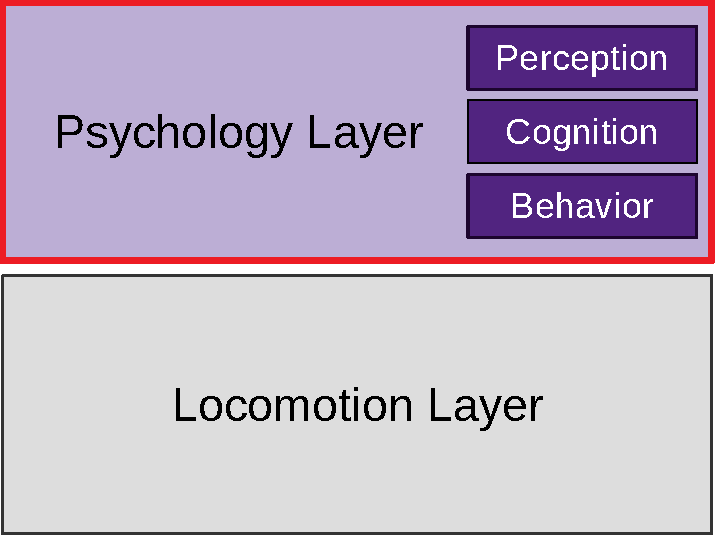
\includegraphics[width=\linewidth]{VaderePsychologyLayer/StepByStep/Vadere-PsychologyLayerDetailed-PsychologyLayerHighlighted}
            \end{figure}
        \end{column}
        \begin{column}[c]{0.5\linewidth}
            \begin{figure}
                \centering
                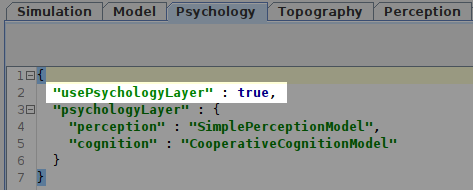
\includegraphics[width=\linewidth]{VaderePsychologyLayer/GUI/Vadere-GUI-PsychologyTab-UsePsychologyLayerHighlighed}
            \end{figure}
        \end{column}
    \end{columns}
    \twocolcaption{}
    
    \note[item]{First of all, the new psychology layer is completely optional and can be enabled/disabled via a simple flag.}
    \note[item]{This decision keeps the simulator backward-compatible to the state before adding a psychology layer.}
    \note[item]{The psychology layer consists of three sequential steps which let agents adapt their behavior.}
\end{frame}

\begin{frame}[c]{Psychology layer: Perception}
    
    \begin{columns}
        \begin{column}[c]{0.5\linewidth}
            \begin{figure}
                \centering
                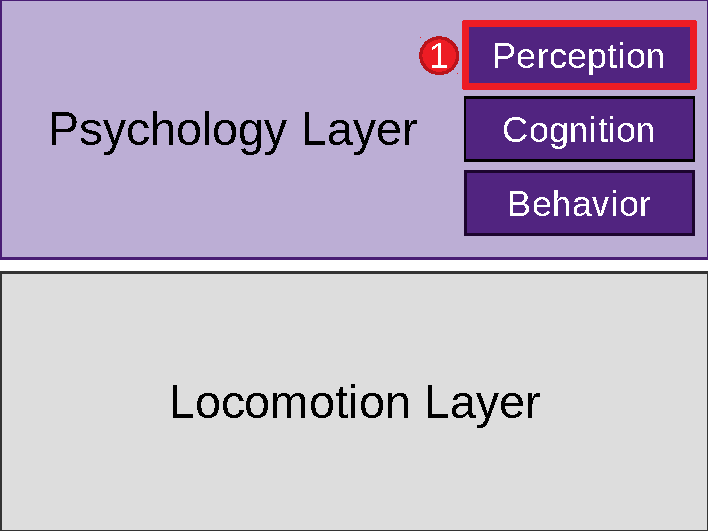
\includegraphics[width=\linewidth]{VaderePsychologyLayer/StepByStep/Vadere-PsychologyLayerDetailed-PerceptionHighlighted}
            \end{figure}
        \end{column}
        \begin{column}[c]{0.5\linewidth}
            \begin{figure}
                \centering
                \only<1>{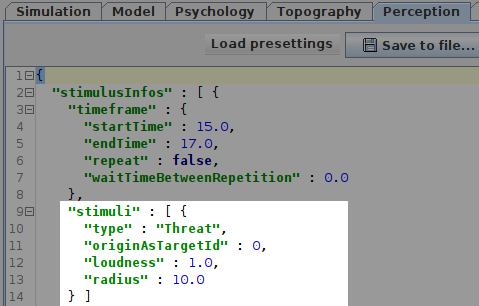
\includegraphics[width=\linewidth]{VaderePsychologyLayer/GUI/Vadere-GUI-PerceptionTab-Highlighted}}
                \only<2>{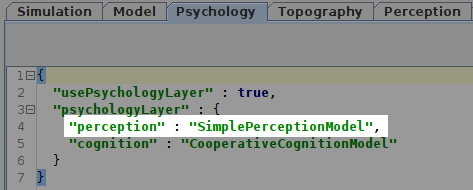
\includegraphics[width=\linewidth]{VaderePsychologyLayer/GUI/Vadere-GUI-PsychologyTab-PerceptionHighlighed}}
                \only<3>{\lstinputlisting[caption={},label={lst:SimplePerceptionModelPseudoCode},language=Java]{Listings/SimplePerceptionModel-PseudoCode.java}}
            \end{figure}
        \end{column}
    \end{columns}
    \twocolcaption{}
    
    \note<1>[item]{When enabled, the user can place environmental stimuli in the simulation area which can be perceived by agents.}
    \note<1>[item]{That means the user can create a list of stimuli for a simulation run.}
    \note<2>[item]{Additionally, the user can define how how these stimuli are prioritized.}
    \note<3>[item]{For instance, if a visual cue like an advertisement and a loud bang occur simultaneously, a perception model can rank these stimuli.}
    \note<3>[item]{A perception model just loops over the available pedestrians and prioritizes stimuli.}
    \note<3>[item]{During the experiment, there were no stimuli. That means, for users, it is completely optional to utilize these layers.}
    
\end{frame}

\begin{frame}[c]{Psychology layer: Cognition}
    
    \begin{columns}
        \begin{column}[c]{0.5\linewidth}
            \begin{figure}
                \centering
                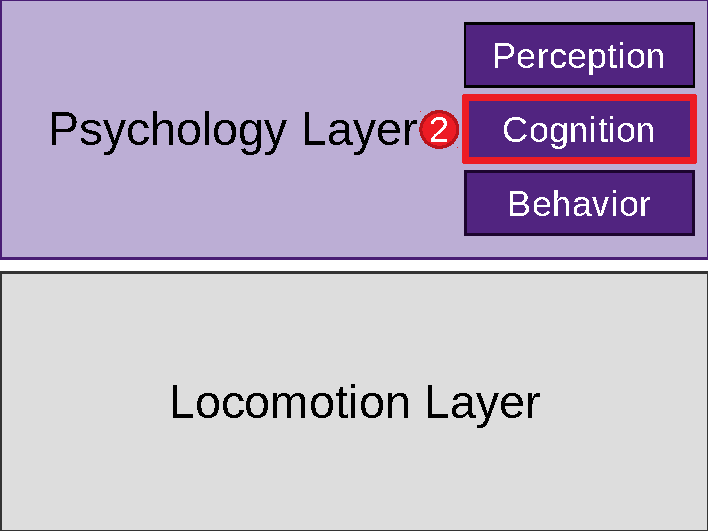
\includegraphics[width=\linewidth]{VaderePsychologyLayer/StepByStep/Vadere-PsychologyLayerDetailed-CognitionHighlighted}
            \end{figure}
        \end{column}
        \begin{column}[c]{0.5\linewidth}
            \begin{figure}
                \centering
                \only<1>{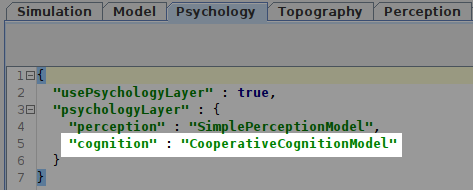
\includegraphics[width=\linewidth]{VaderePsychologyLayer/GUI/Vadere-GUI-PsychologyTab-CognitionHighlighed}}
                \only<2>{\lstinputlisting[caption={},label={lst:CooperativeCognitionModelPseudoCode},language=Java]{Listings/Cognition-CooperativeCognitionModel-PseudoCode.java}}
            \end{figure}
        \end{column}
    \end{columns}
    \twocolcaption{}
    
    \note[item]{Additionally, the user can configure the cognitive abilities of the agents in the cognition layer.}
    \note[item]{For our experiment, this means that agents get cooperative and let walking agents through.}
    \note[item]{It requires only 13 lines of code with the new psychology layer to allow simple behavioral changes.}    
    
\end{frame}

\begin{frame}[c]{Psychology layer: Behavior}
    
    \begin{columns}
        \begin{column}[c]{0.5\linewidth}
            \begin{figure}
                \centering
                \only<1>{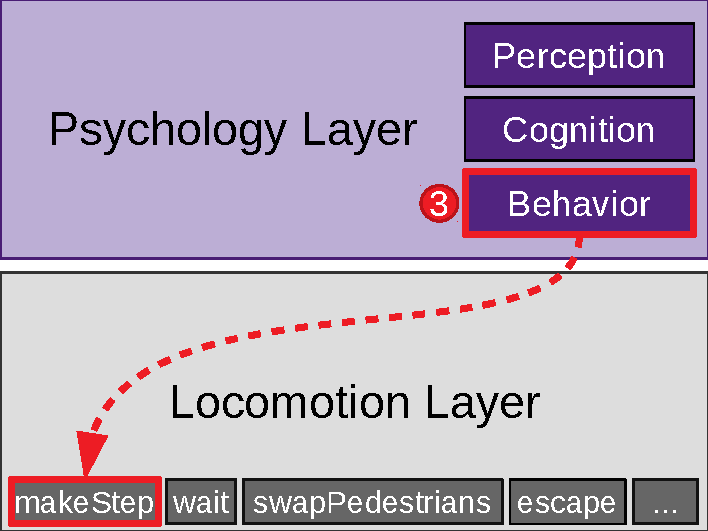
\includegraphics[width=\linewidth]{VaderePsychologyLayer/StepByStep/Vadere-PsychologyLayerDetailed-BehaviorMakeStepHighlighted}}
                \only<2>{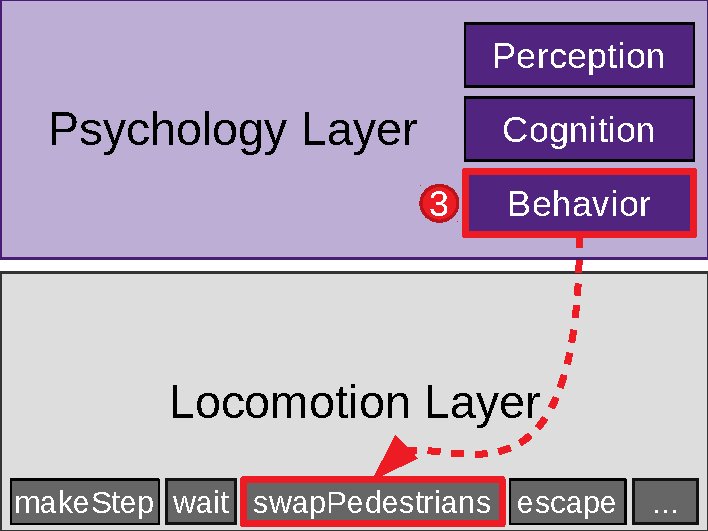
\includegraphics[width=\linewidth]{VaderePsychologyLayer/StepByStep/Vadere-PsychologyLayerDetailed-BehaviorSwapPedestrians}}
            \end{figure}
        \end{column}
        \begin{column}[c]{0.5\linewidth}
            \begin{figure}
                \centering
                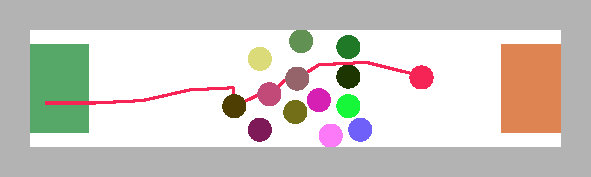
\includegraphics[width=\linewidth]{VaderePsychologyLayer/DisabledVsEnabled/CooperativeCognitionModel-PsychEnabled}
                \newline
                {\footnotesize ...towards cooperation.}
                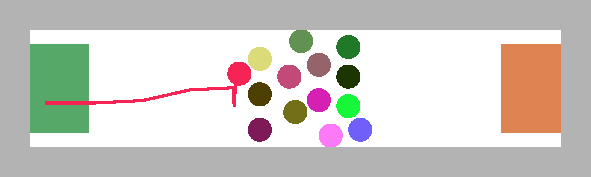
\includegraphics[width=\linewidth]{VaderePsychologyLayer/DisabledVsEnabled/CooperativeCognitionModel-PsychDisabled}
                \newline
                {\footnotesize Behavioral change...}
            \end{figure}
        \end{column}
    \end{columns}
    \twocolcaption{}
    
    \note[item]{The last crucial step to allow behavioral changes is to equip agents with a behavioral repertoire instead of having only one movement strategy. That is, walking towards a target.}
    
\end{frame}

\begin{frame}{Foundations}
    
    My research is based on three pillars:
    \vspace{-\baselineskip}
    % Text is placed in three columns. Images follow also in three colums but on own line.
    \begin{columns}
        \begin{column}[t]{0.36\textwidth}
            \begin{block}{Experiment}
                \vspace{-0.5\baselineskip}
                \begin{itemize}
                    \item In Oct 2018 with 58 participants
                    \item To re-enact \enquote{failing} simulation from previous slides
                \end{itemize}
            \end{block}
        \end{column}
        \begin{column}[t]{0.40\textwidth}
            \begin{block}{OPMOPS project}
                \vspace{-0.5\baselineskip}
                \begin{itemize}
                    \item Franco-German project about demonstrations in urban areas.
                    \item Goal: Implement a \enquote{decision support system} to plan and handle events.
                \end{itemize}
            \end{block}
        \end{column}
        \begin{column}[t]{0.36\textwidth}
            \begin{block}{Research stay in UK}
                \vspace{-0.5\baselineskip}
                \begin{itemize}
                    \item At University of Sussex
                    \item Exchange with social psychology professor Dr. John Drury and his team
                \end{itemize}
            \end{block}
        \end{column}
    \end{columns}
    \vspace{-0.30\baselineskip}
    \begin{columns}
        \begin{column}[t]{0.36\textwidth}
            \centering
            \href{run:./Videos/Experiment.mp4}{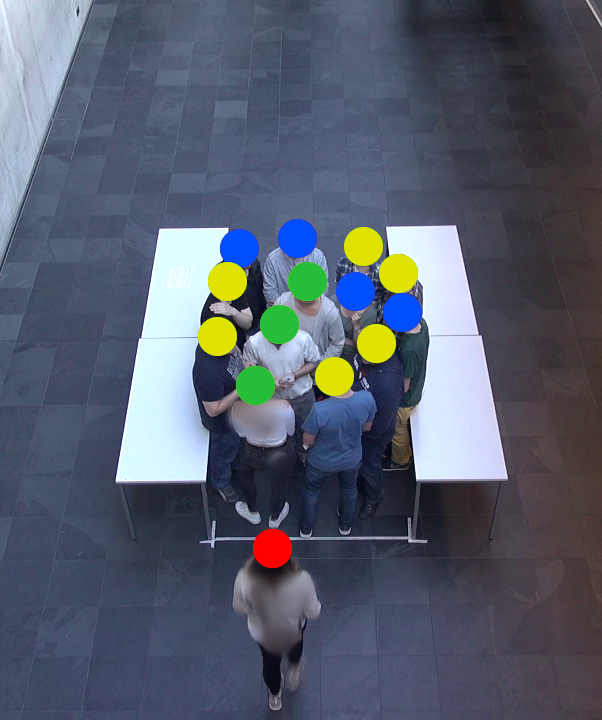
\includegraphics[height=0.30\textheight]{Psychology/ExperimentDenseCrowd/Experiment-DenseCrowd-VideoFootage-Modified}}
        \end{column}
        \begin{column}[t]{0.40\textwidth}
            \centering
            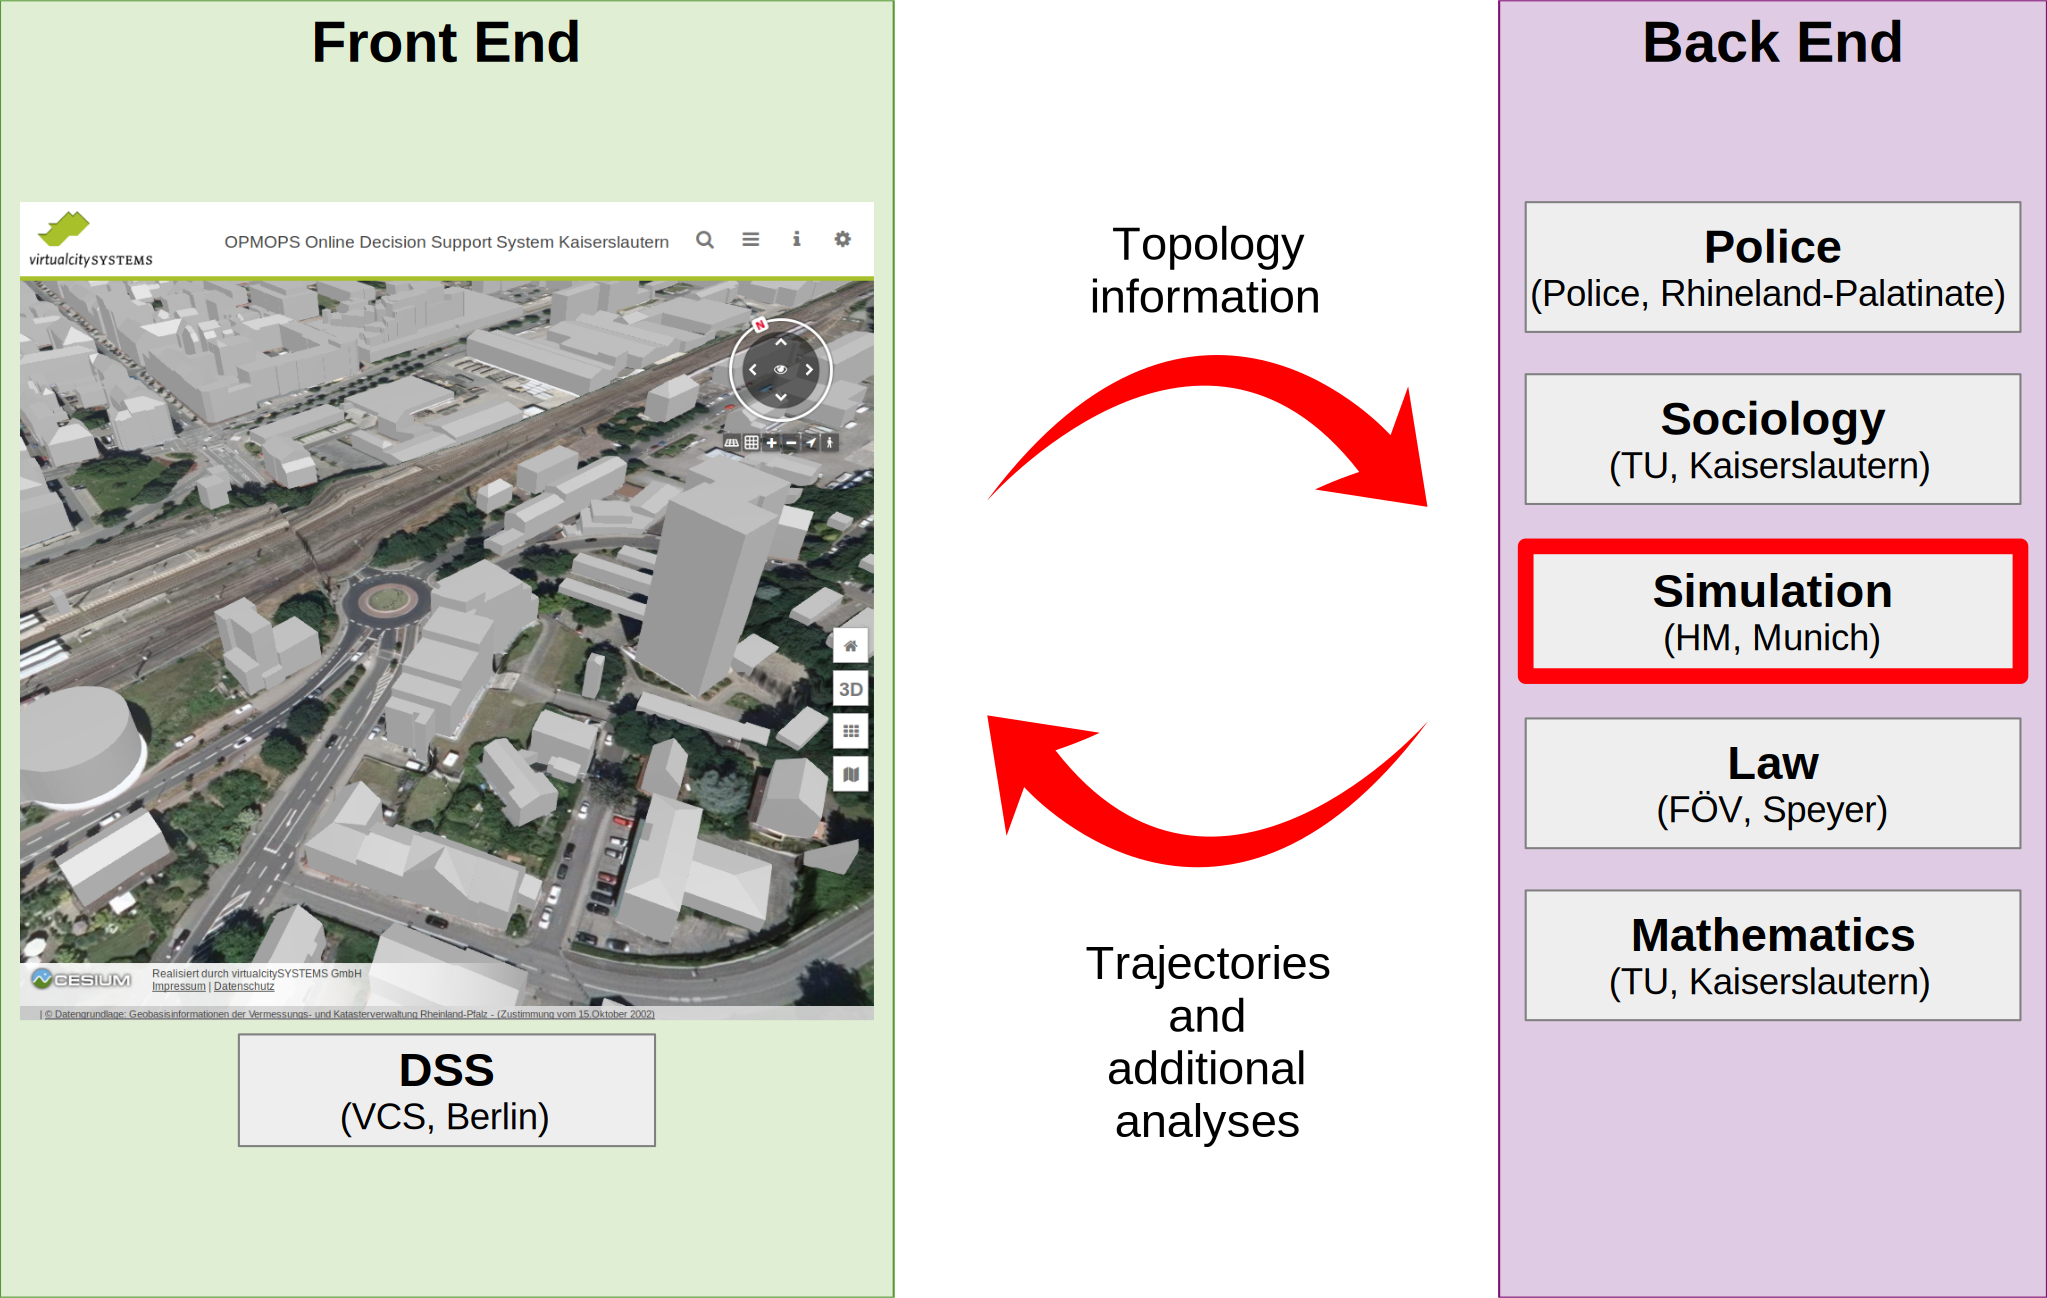
\includegraphics[height=0.30\textheight]{Psychology/DSSInteraction/DSS-Interaction-BackEnd2}
        \end{column}
        \begin{column}[t]{0.36\textwidth}
            \centering
            
\includegraphics[height=0.30\textheight]{Psychology/ResearchStay/University_of_Sussex_Logo}
        \end{column}
    \end{columns}
    
\end{frame}

% TODO Mention contributions: psychology layer, simulator maintenance, OpenStreetMap importer, CI/CD to Vadere website
\begin{frame}{Summary}
    \scriptsize
    \begin{columns}[T]
        \column{0.45\textwidth}
        \begin{minipage}[c][0.4\textheight][t]{\textwidth}
            \visible<1->{
            \begin{block}{Research question:}
                \scriptsize
                \ResearchQuestion{}
            \end{block}
            }
            \visible<1->{
            \begin{block}{My proposal:}
                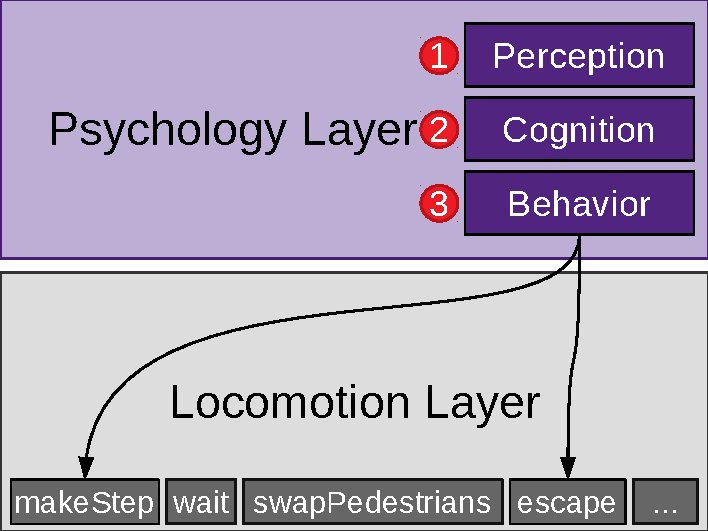
\includegraphics[width=\textwidth]{VaderePsychologyLayer/StepByStep/Vadere-PsychologyLayerDetailed}
            \end{block}
            }
        \end{minipage}
        \column{0.55\textwidth}
        \begin{minipage}[c][0.4\textheight][t]{\textwidth}
            \begin{block}{Contributions:}
                \begin{enumerate}
                    \scriptsize
                \visible<2->{
                    \item Integrated psychology layer
                    \begin{itemize}
                        \scriptsize
                        \item based on empirical data (own experiment)
                        \item tested by practitioners (police Rhineland-Palatinate)
                        \item operationalized behavioral changes with social psychologists
                    \end{itemize}
                }
                \visible<3->{
                    \scriptsize
                    \item Software engineering
                    \begin{itemize}
                        \scriptsize
                        \item I encapsulated my approach as reusable psychology layer (for other simulators)
                        \item Set up CI/CD to deploy Vadere simulator to website
                        \item Simulator maintenance (GUI, OpenStreetMap converter, ...)
                    \end{itemize}
                    All source code contributions are open source: \url{https://gitlab.lrz.de/vadere/vadere}
                }
                \end{enumerate}
                \vspace{-4mm}
            \end{block}
        \end{minipage}
    \end{columns}

    \note<1>[item]{Now, let's wrap up my presentation and come to the conclusions.}
    \note<1>[item]{Because of the scientific gap, I posed the research question of \enquote{\ResearchQuestion{}}}
    \note<2>[item]{My proposal is a reusable psychology layer with three sequential phases: perception, cognition and a behavioral selection.}
    \note<2>[item]{I based my work on three pillars beside an exhaustive literature research: an own experiment, a research stay with social psychologists and three validation use cases.}
    \note<2>[item]{In my experiment I collected qualitative and quantitative data about human behavior. This data is useful for the whole research community and my approach is based on empirical data.}
    \note<2>[item]{I included social psychologists in my research.}
    
\end{frame}

\setbeamertemplate{footline}{} % remove footer for the last slide
\appendix % end counting

\begin{frame}
\label{BackupSlides}

    \begin{center}
        \Huge
        \vfill
        Backup slides
        \vfill
    \end{center}
    \begin{center}
        \hyperlink{Backup:SimulatorDetails}{\beamerbutton{Simulator details}} \(\cdot\) \hyperlink{Backup:SimulationResults}{\beamerbutton{Simulation results}} \(\cdot\) \hyperlink{Backup:NavigationAndWayfinding}{\beamerbutton{Navigation and wayfinding}}
    \end{center}
\end{frame}

\begin{frame}{Vadere: Core features \hfill \hyperlink{BackupSlides}{\beamerbutton{Back}}}
\label{Backup:SimulatorDetails}

    \begin{columns}
        \begin{column}{0.45\textwidth}
            \begin{itemize}
                \item<1-> Easy-to-use GUI
                \item<2-> CLI for automation
                \item<3-> Shipped with different locomotion models:
                \begin{itemize}
                    \item<3-> Mature: Optimal steps model (OSM), social force model (SFM), ...
                    \item<3-> Experimental: Behavioral heuristics model (BHM), Reynolds' steering, ...
                \end{itemize}
                \item<4-> JSON-based input files
                \item<5-> Continuous integration / deployment pipeline
            \end{itemize}
        \end{column}
        \begin{column}{0.45\textwidth}
            \vspace*{-1.5ex}
            \only<1,3>{
                \begin{figure}
                    \centering
                    \begin{subfigure}{\textwidth}
                        \centering
                        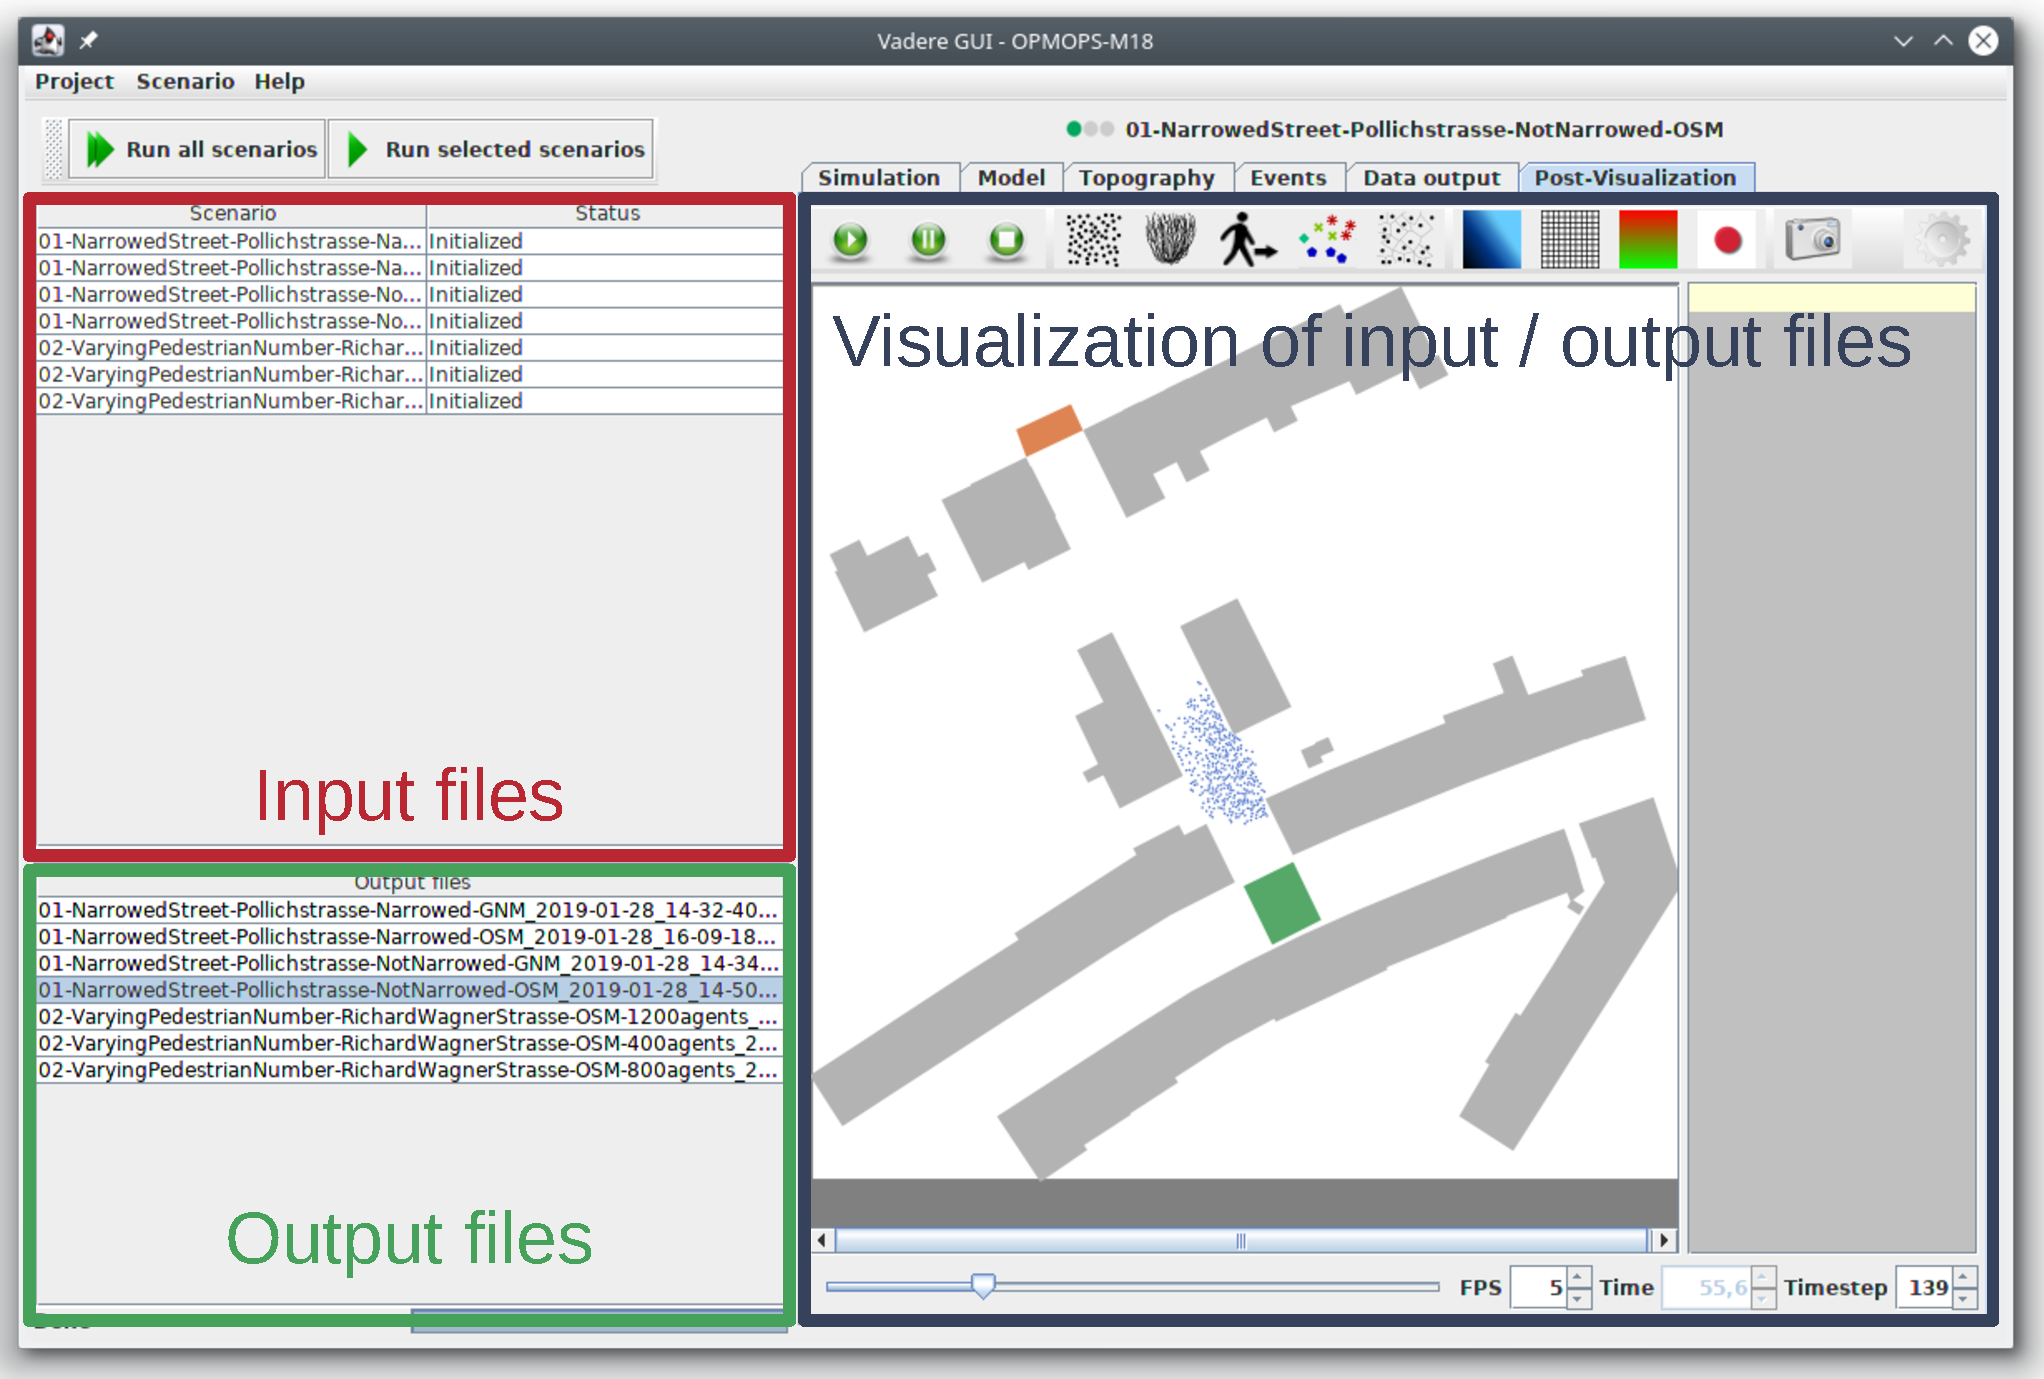
\includegraphics[width=\textwidth]{VadereFeatures/GUI-OnlineVisualization-WithDescription}
                    \end{subfigure}\\
                    \caption{Vadere GUI features}
                    \begin{subfigure}{0.475\textwidth}
                        \centering
                        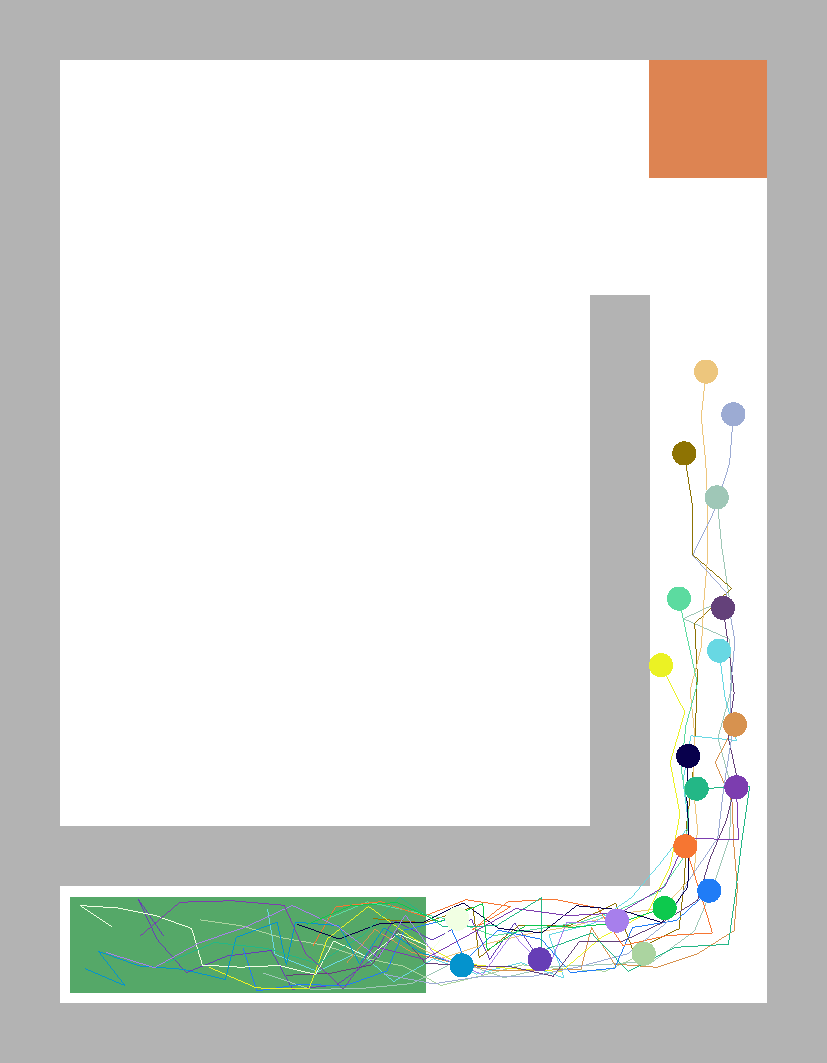
\includegraphics[width=\textwidth]{VadereFeatures/Vadere-PostVisualization-ColoredAgents}
                    \end{subfigure}
                    \begin{subfigure}{0.475\textwidth}
                        \centering
                        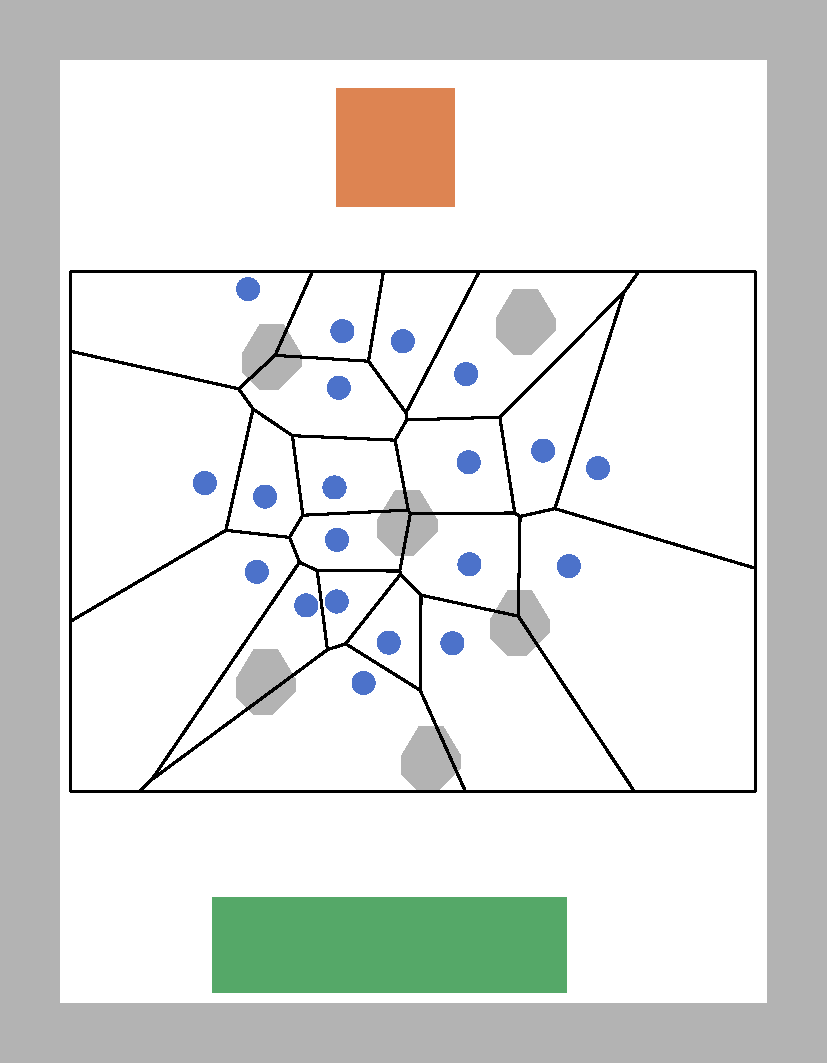
\includegraphics[width=\textwidth]{VadereFeatures/Vadere-PostVisualization-VoronoiDiagram}
                    \end{subfigure}
                    \label{fig:VadereScreenshots}
                \end{figure}
            }
            \only<2>{
                \begin{figure}
                    \lstinputlisting[caption={Vadere's command line interface (CLI)},label={lst:RunVadereConsole},language=bash]{Listings/run_vadere_console.txt}
                \end{figure}
            }
            \only<4>{
                \begin{figure}
                    \lstinputlisting[caption={},label={lst:VadereJsonInputFile},language=Python]{Listings/chicken_floorfield_ok.scenario}
                \end{figure}
            }
            \only<5>{
                \begin{figure}
                    \centering
                    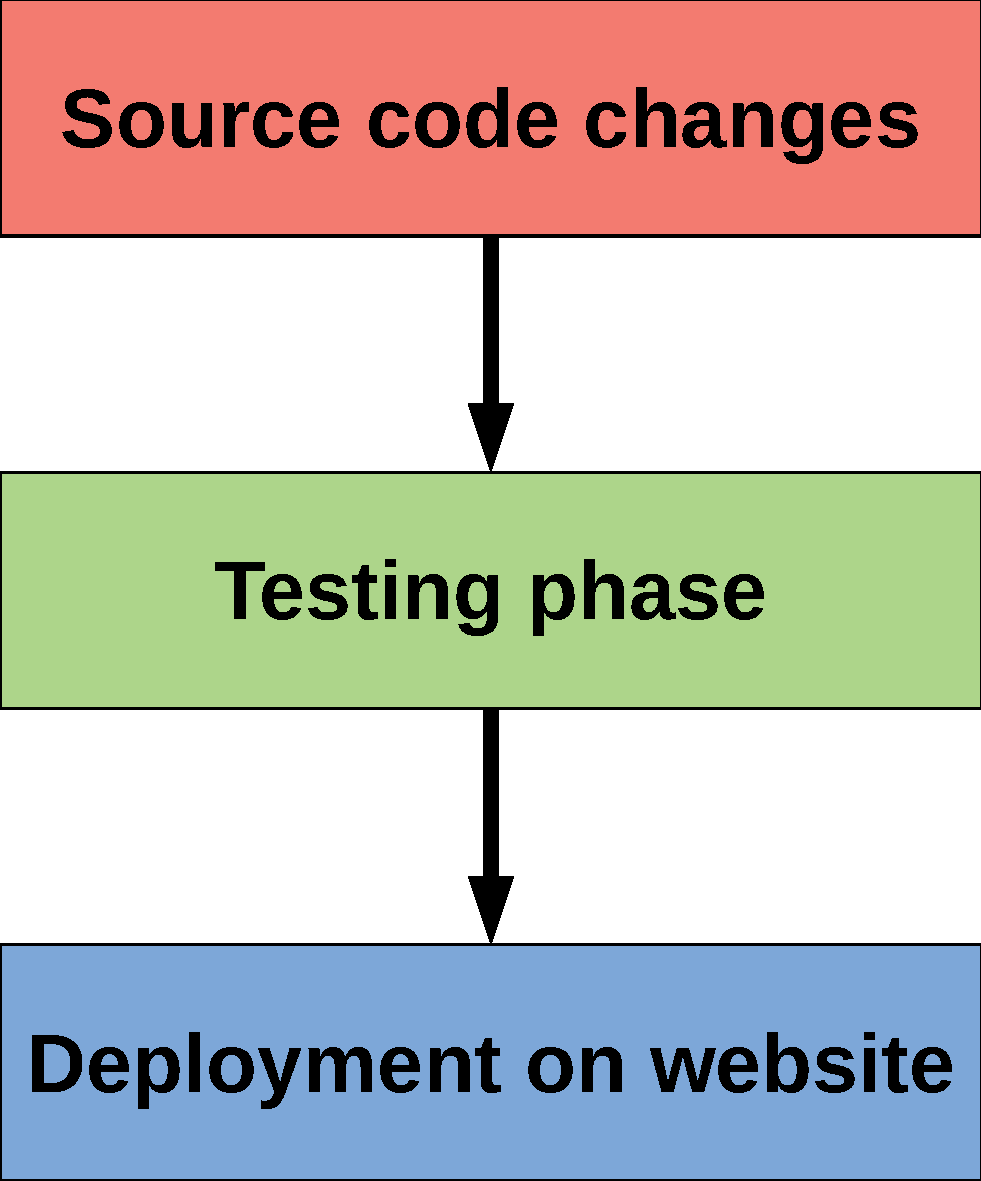
\includegraphics[width=0.8\textwidth]{ContinuousIntegration/CI-Steps}
                    \caption{Continuous integration pipeline}
                    \label{fig:CISteps}
                \end{figure}
            }
        \end{column}
    \end{columns}
    
\end{frame}

\begin{frame}{Getting started}
    
    \begin{enumerate}
        
        \item Download Vadere from: \url{http://www.vadere.org/releases/} 
        \item Unzip package from (1)
        \item Run: \textbf{\texttt{[path/to/java] -jar vadere-gui.jar}}
        \item In GUI, open one of the packaged demo scenarios
    \end{enumerate}
    
\end{frame}

\begin{frame}{Simulation results \hfill \hyperlink{BackupSlides}{\beamerbutton{Back}}}
\label{Backup:SimulationResults}

    I used three real-world use cases for validation:
    \begin{enumerate}
        \item Experiment: cooperative behavior
        \item Perceived threat: fleeing and imitation behavior
        \item Counterflowing agents: evasion behavior
    \end{enumerate}

    \begin{center}
        \includegraphics[width=\textwidth]{Implementation/PsychologyLayer/ModelingProcessOutput/PsychologyLayer-InfluencesAndModel-Landscape-04}
    \end{center}
    
    \note[item]{I used three real-world examples to show that the psychology layer is able to...}
    \note[item]{...easily reenact real crowd behavior}
    \note[item]{...with minimal programming overhead}
    \note[item]{The validation --- which is described in more detail in the dissertation --- shows that I combined existing locomotion strategies with essential psychological aspects that affect crowd behavior.}
    \note[item]{Lastly, I would like to dive into a more complex use case where people where fleeing and others imitated this behavior.}
\end{frame}

\begin{frame}{Perceived threat: Simulation setup}
    \begin{columns}[T]
        \column{0.5\textwidth}
        \begin{minipage}[c][0.4\textheight][t]{\textwidth}
            \begin{itemize}
                \item<1-> Real-world incident: stampede after false alarm
                \begin{enumerate}
                    \item<1-> People left underground station target-oriented
                    \item<2-> After bang, people were fleeing
                    \item<3-> Then, they were searching for a safe zone
                    \item<4->  In-group members imitated fleeing behavior \\ \(\rightarrow\) Self-categorization theory (social psychology)
                \end{enumerate}
                \item<4-> Tools:
                \begin{itemize}
                    \item<4-> OpenStreetMap material
                    \item<5-> Vadere simulator with new psychology layer
                \end{itemize}
            \end{itemize}
        \end{minipage}
        \column{0.5\textwidth}
        \begin{minipage}[c][0.4\textheight][t]{\textwidth}
            \centering
            \only<4>{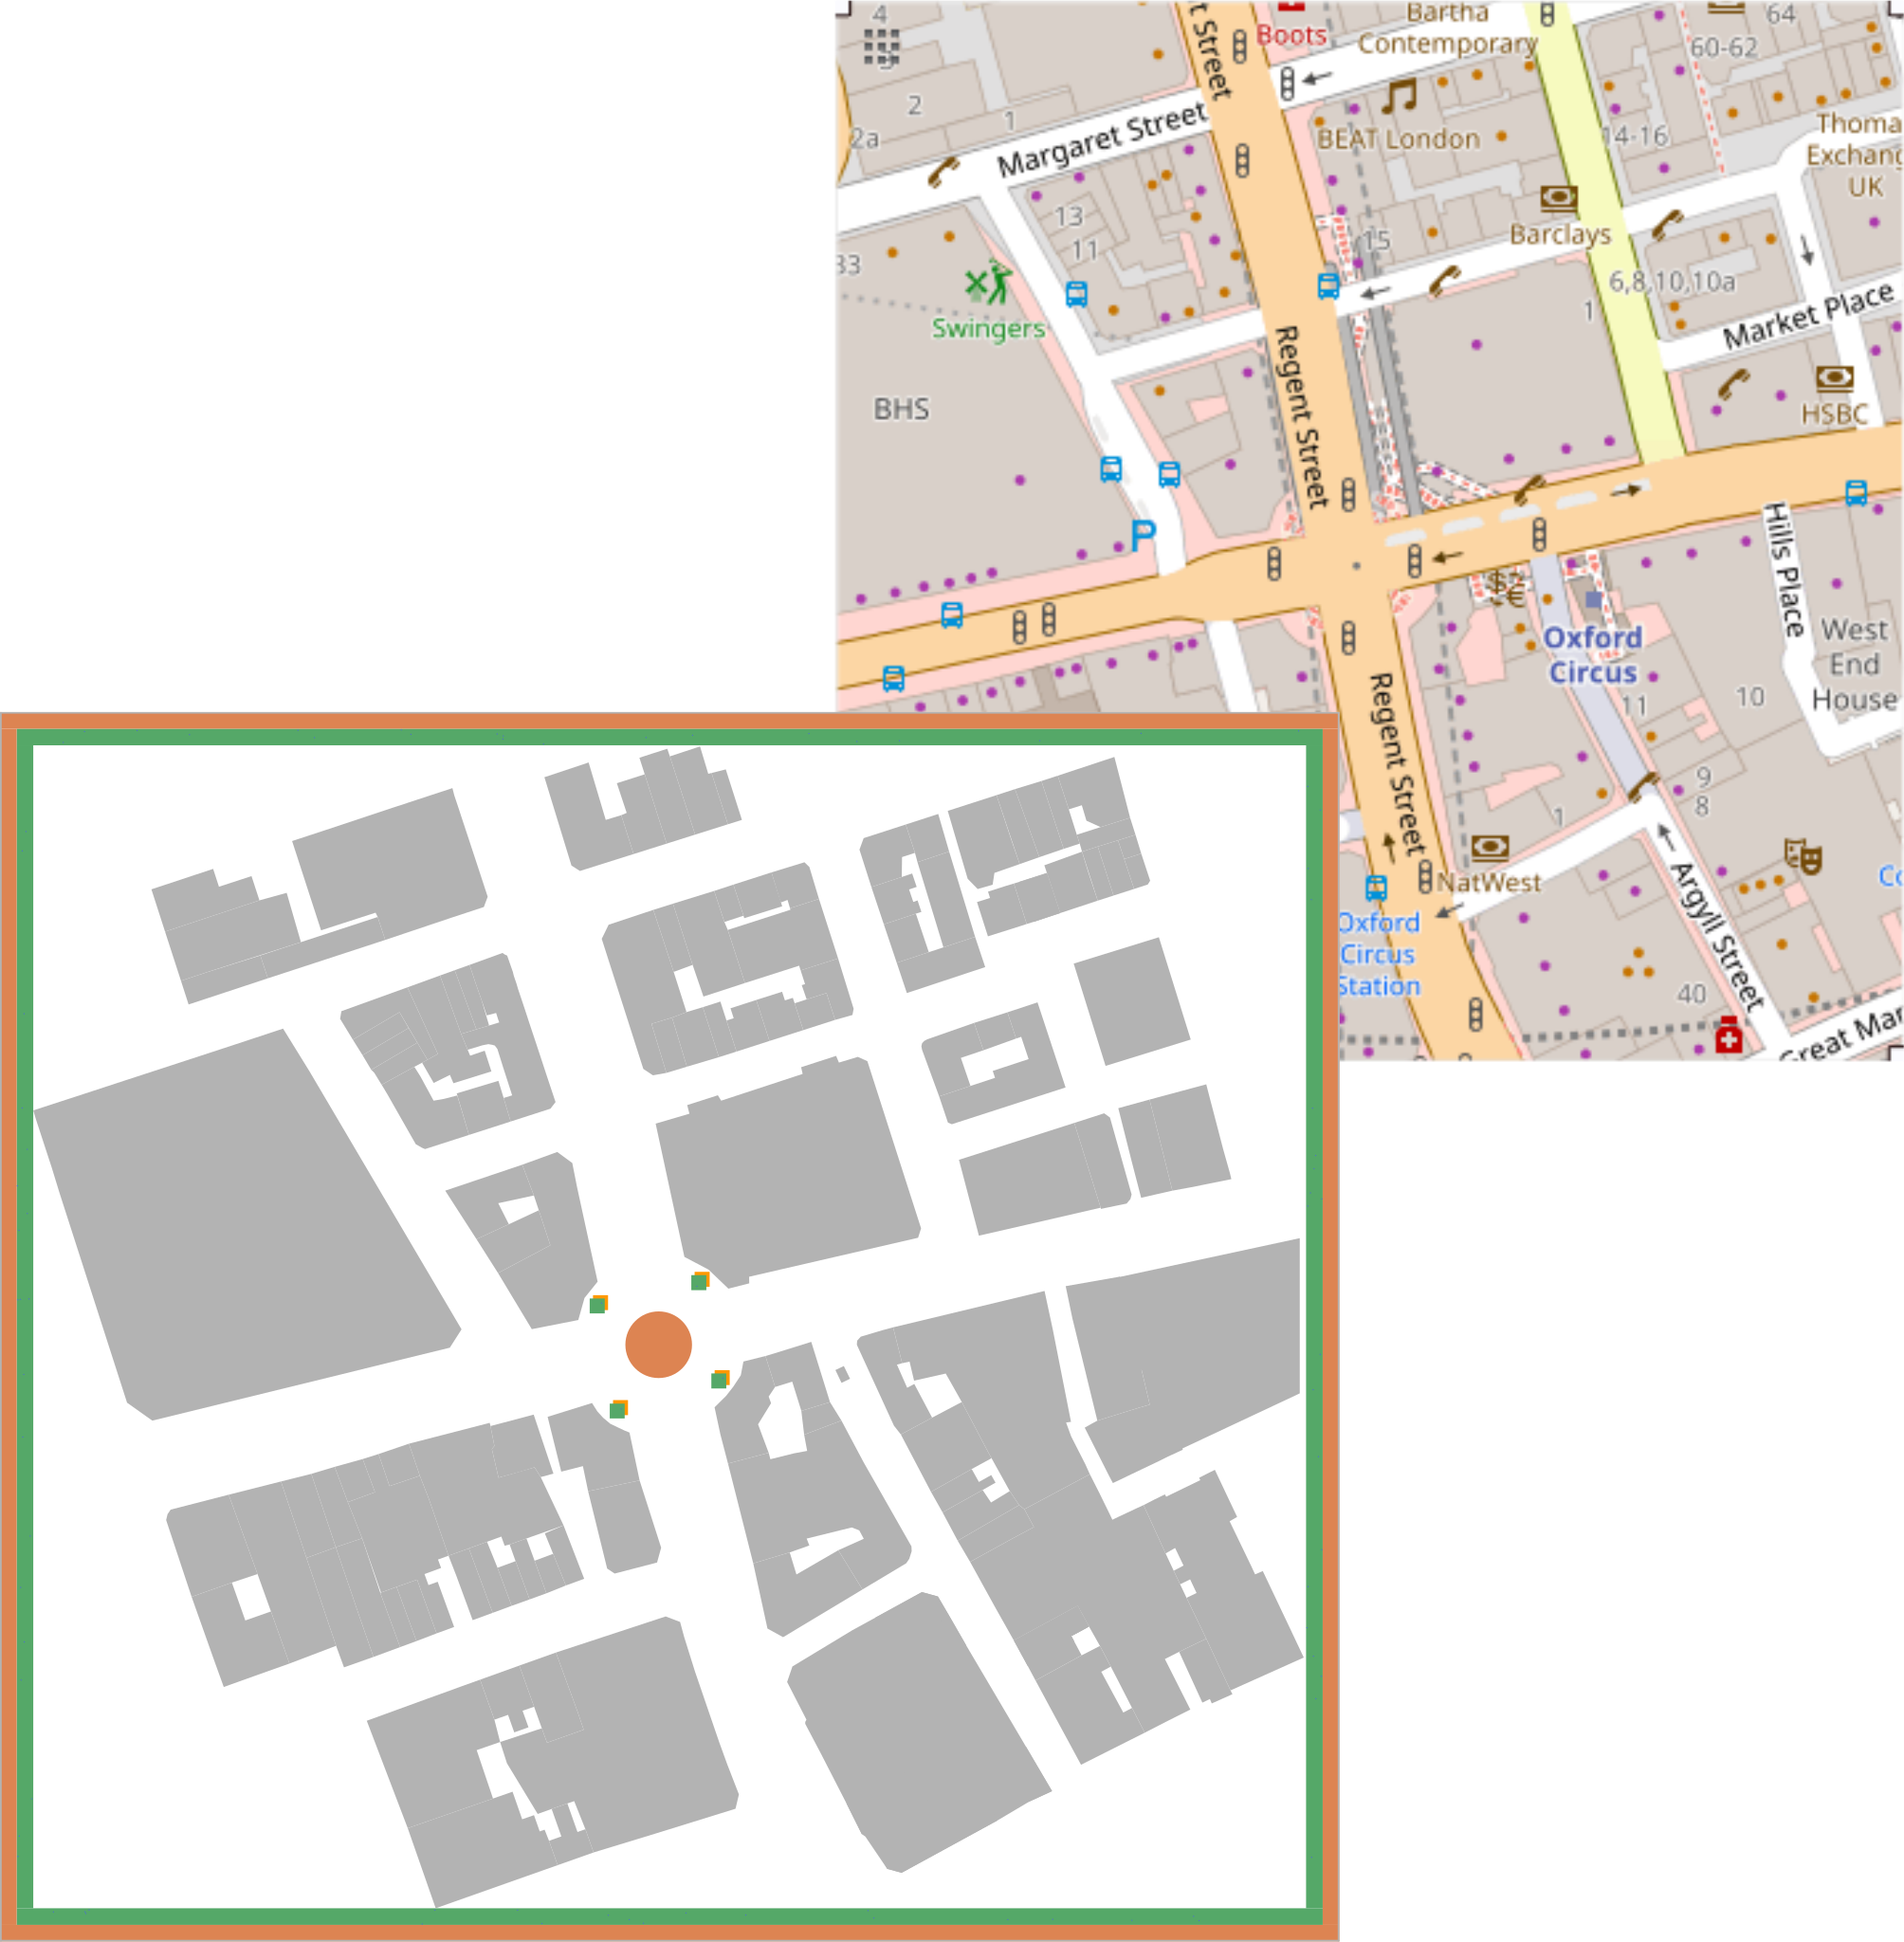
\includegraphics[width=\textwidth]{UseCasesAndValidation/SelfCatThreatModel/OpenStreetMap/SimulationArea-01}}
            \only<5>{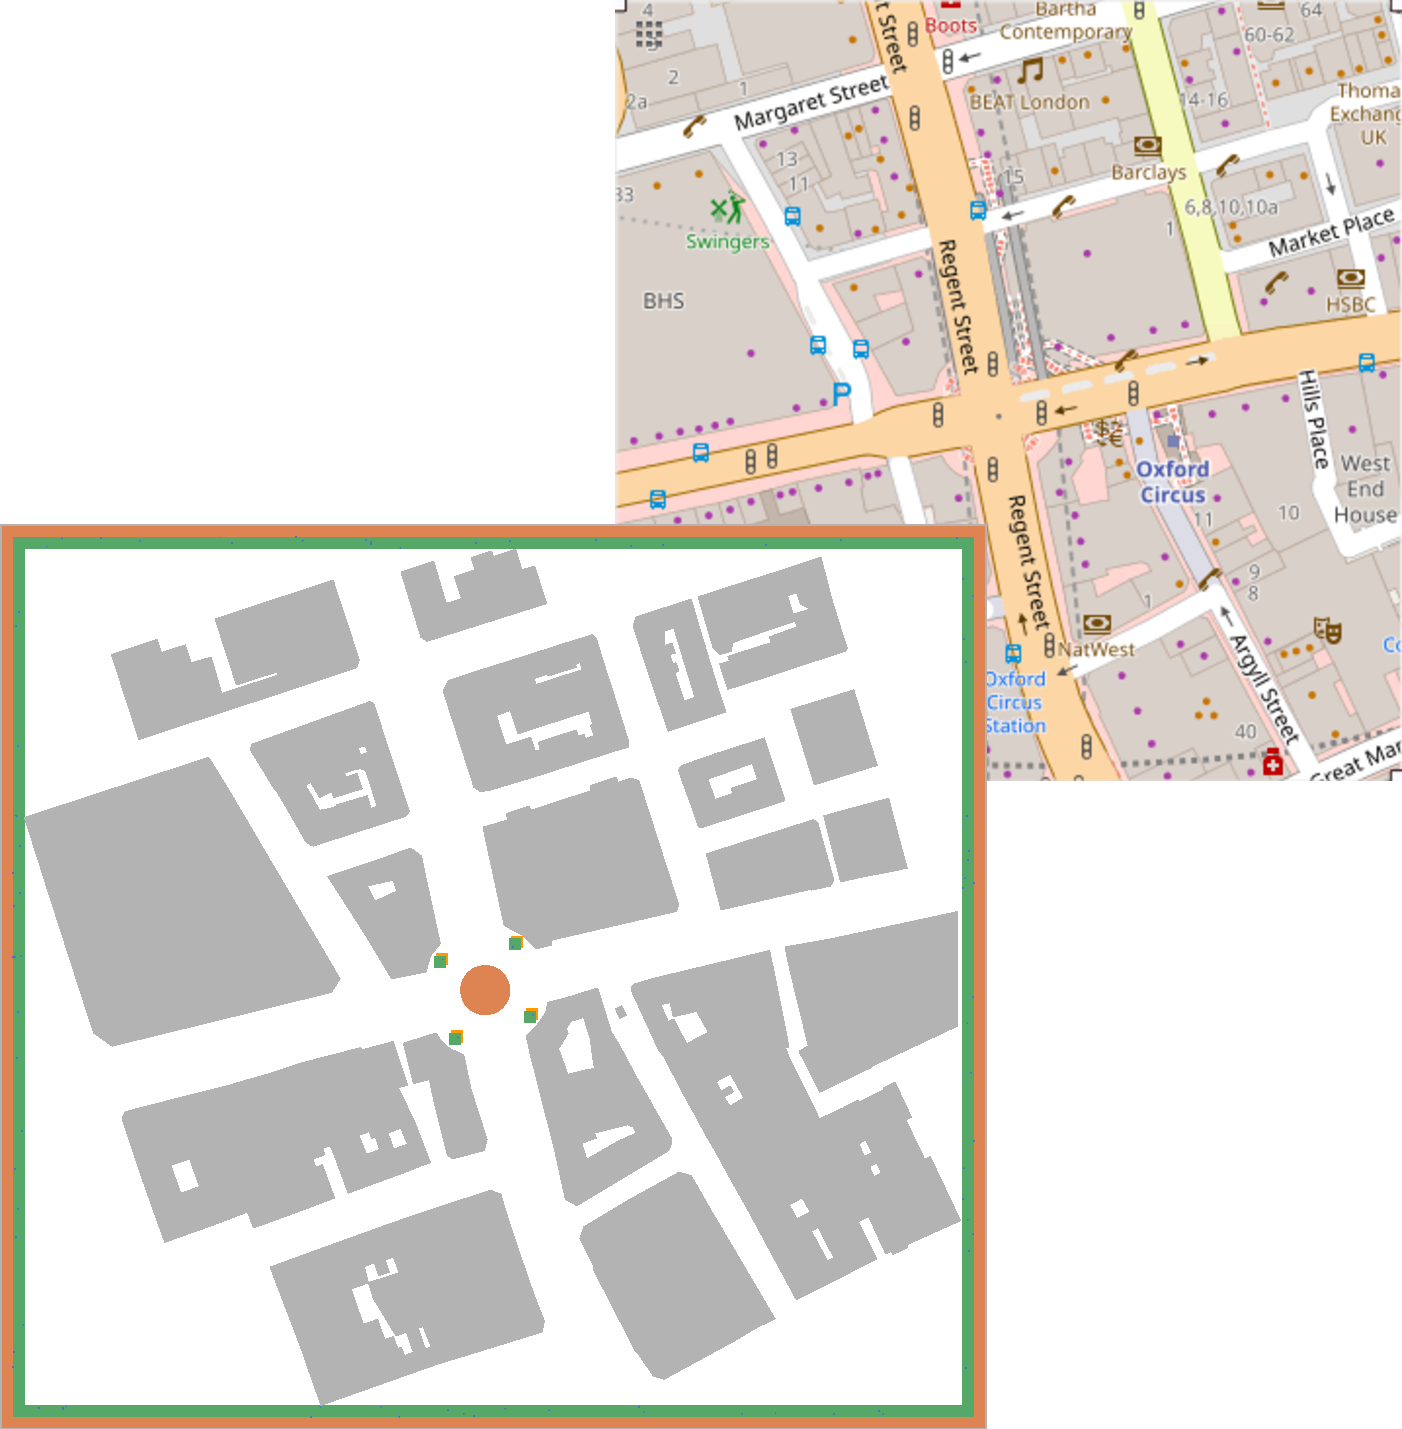
\includegraphics[width=\textwidth]{UseCasesAndValidation/SelfCatThreatModel/OpenStreetMap/SimulationArea-02}}
            \only<6>{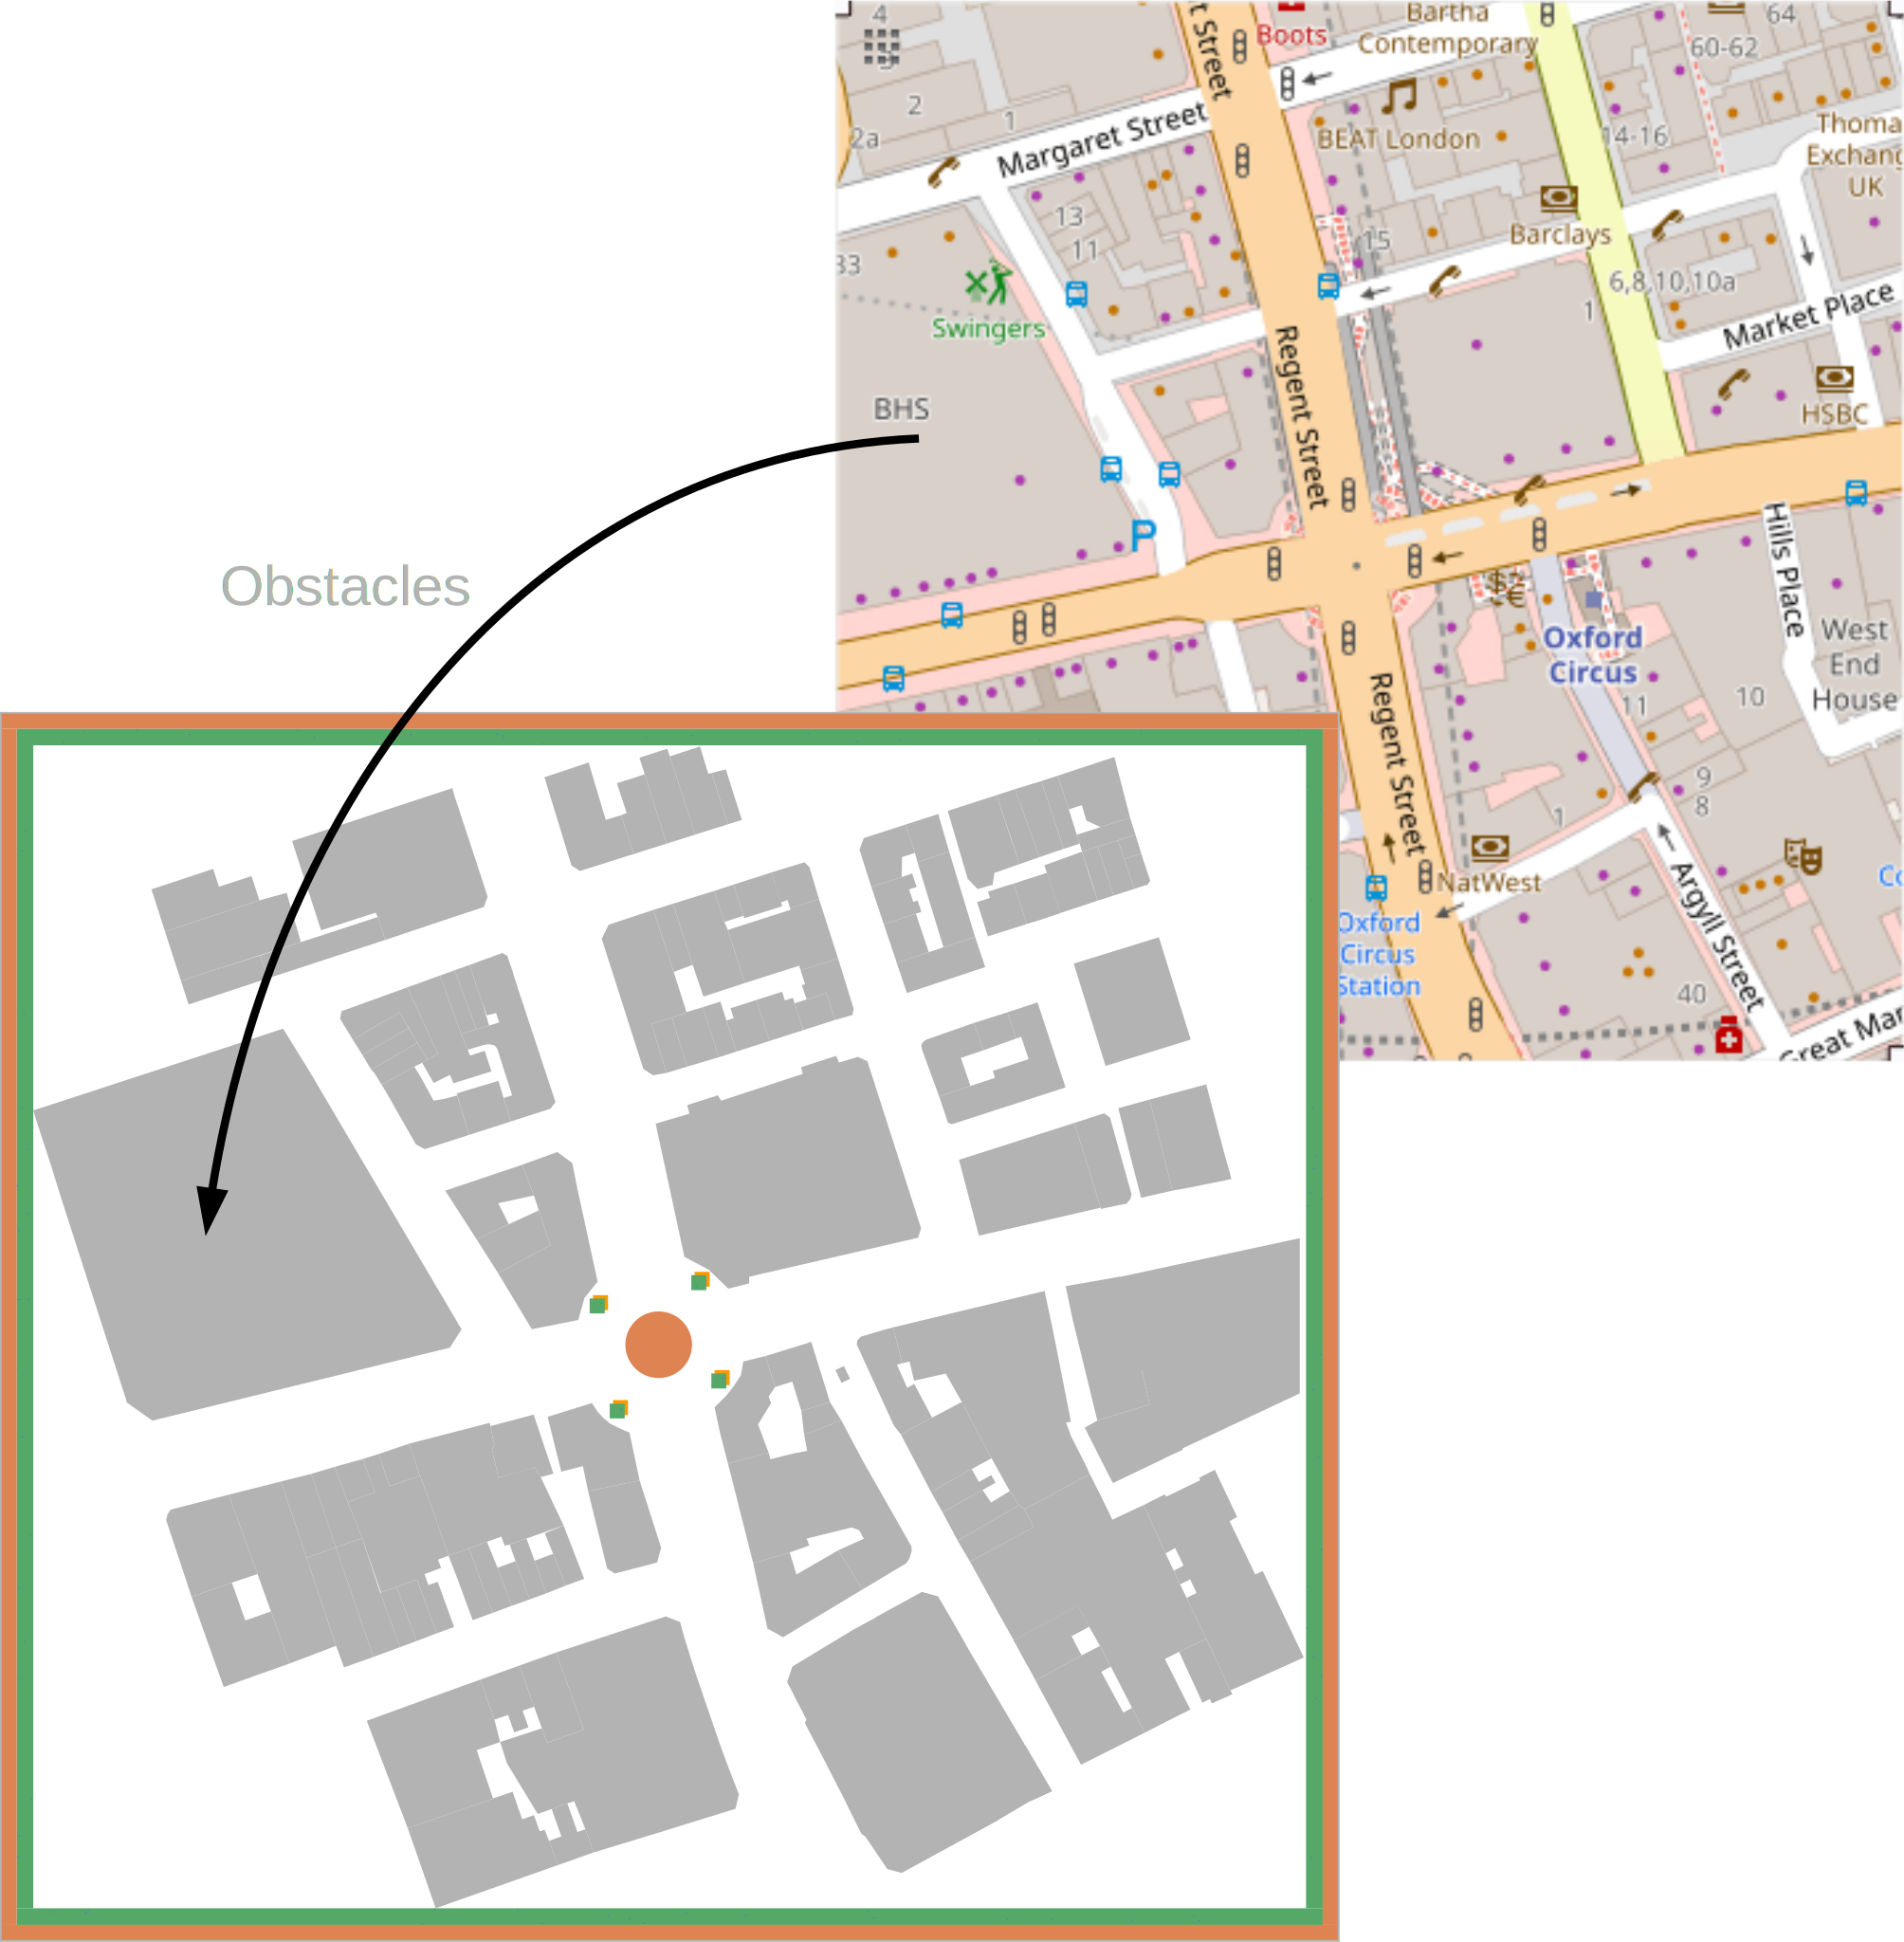
\includegraphics[width=\textwidth]{UseCasesAndValidation/SelfCatThreatModel/OpenStreetMap/SimulationArea-03}}
            \only<7>{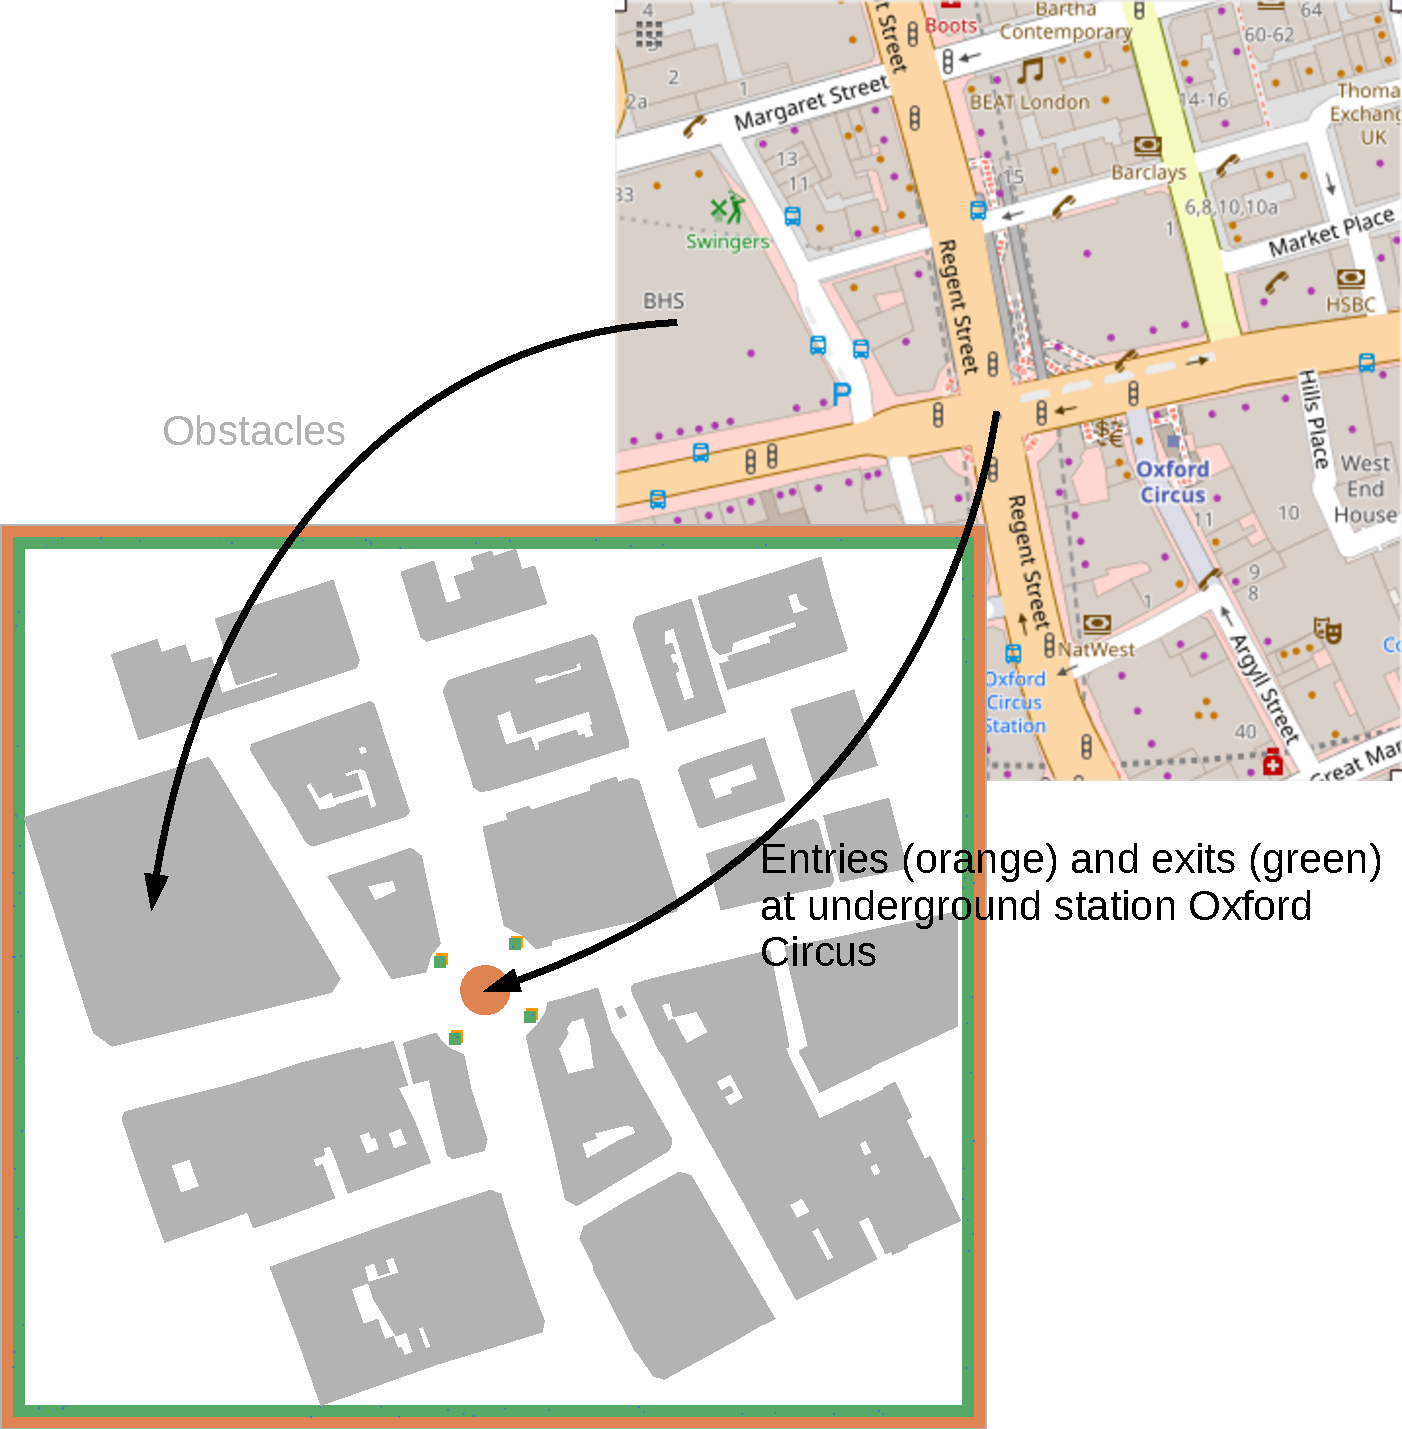
\includegraphics[width=\textwidth]{UseCasesAndValidation/SelfCatThreatModel/OpenStreetMap/SimulationArea-04}}
            \only<8>{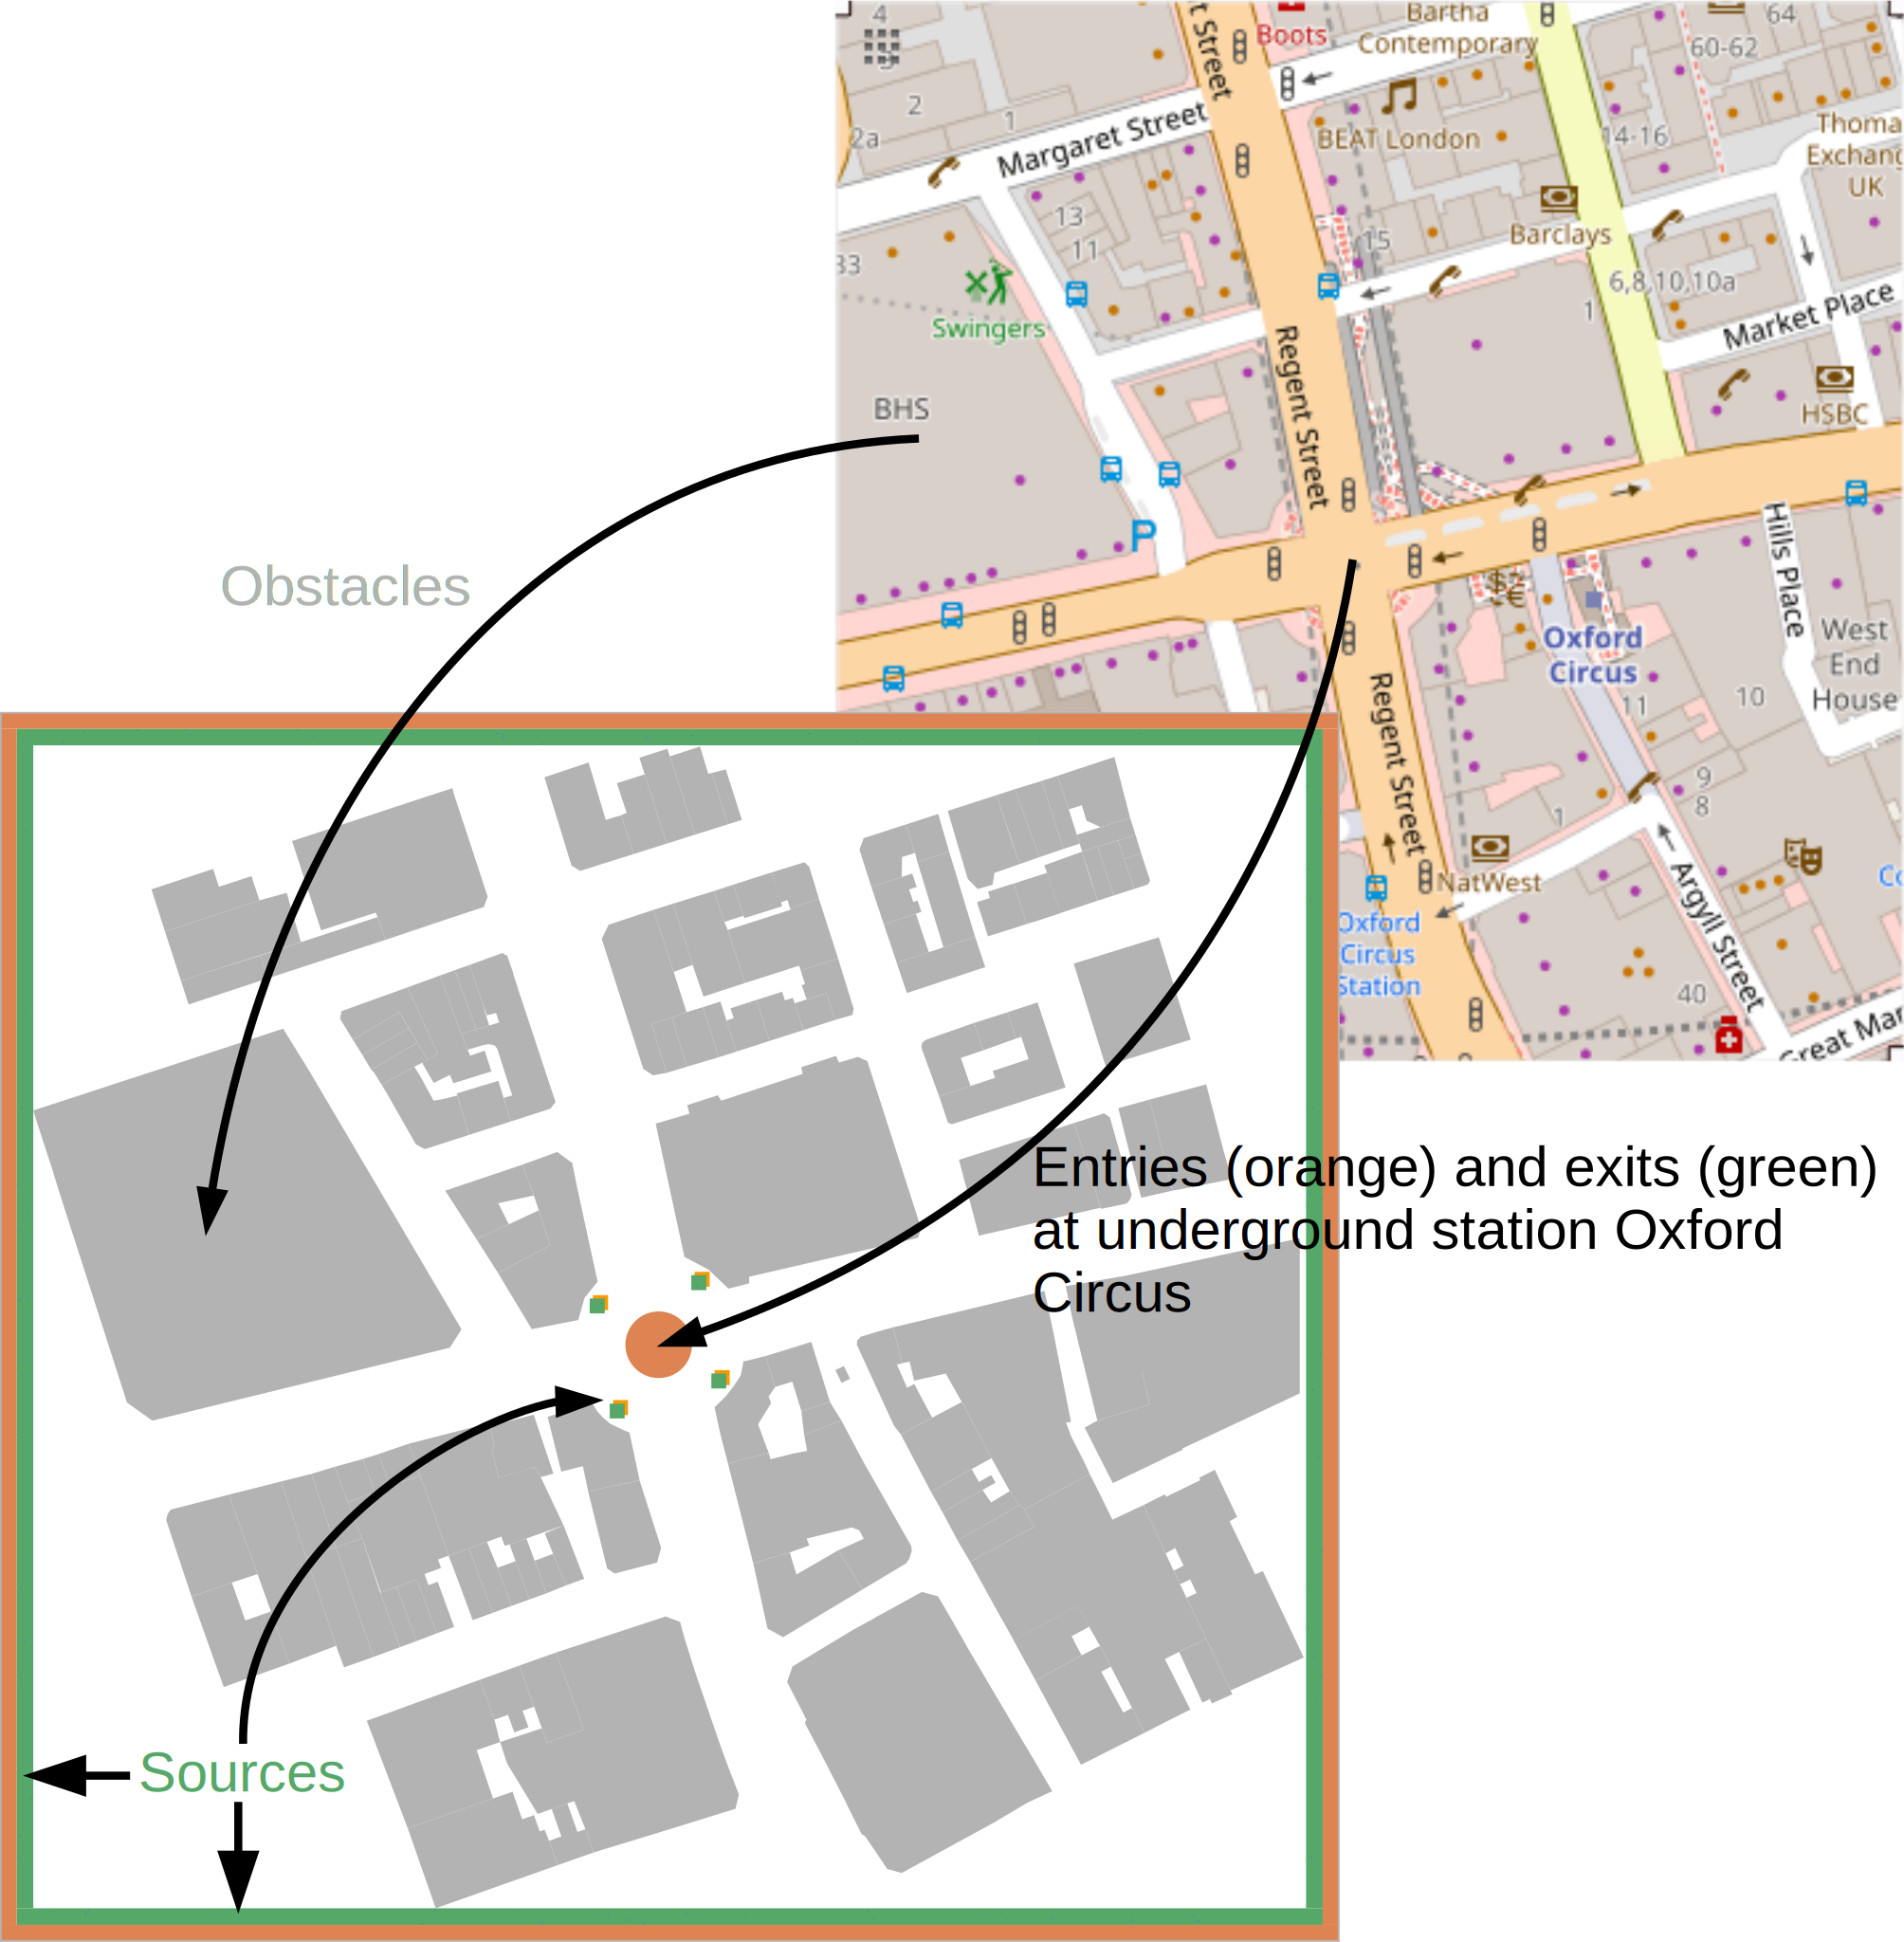
\includegraphics[width=\textwidth]{UseCasesAndValidation/SelfCatThreatModel/OpenStreetMap/SimulationArea-05}}
            \only<9>{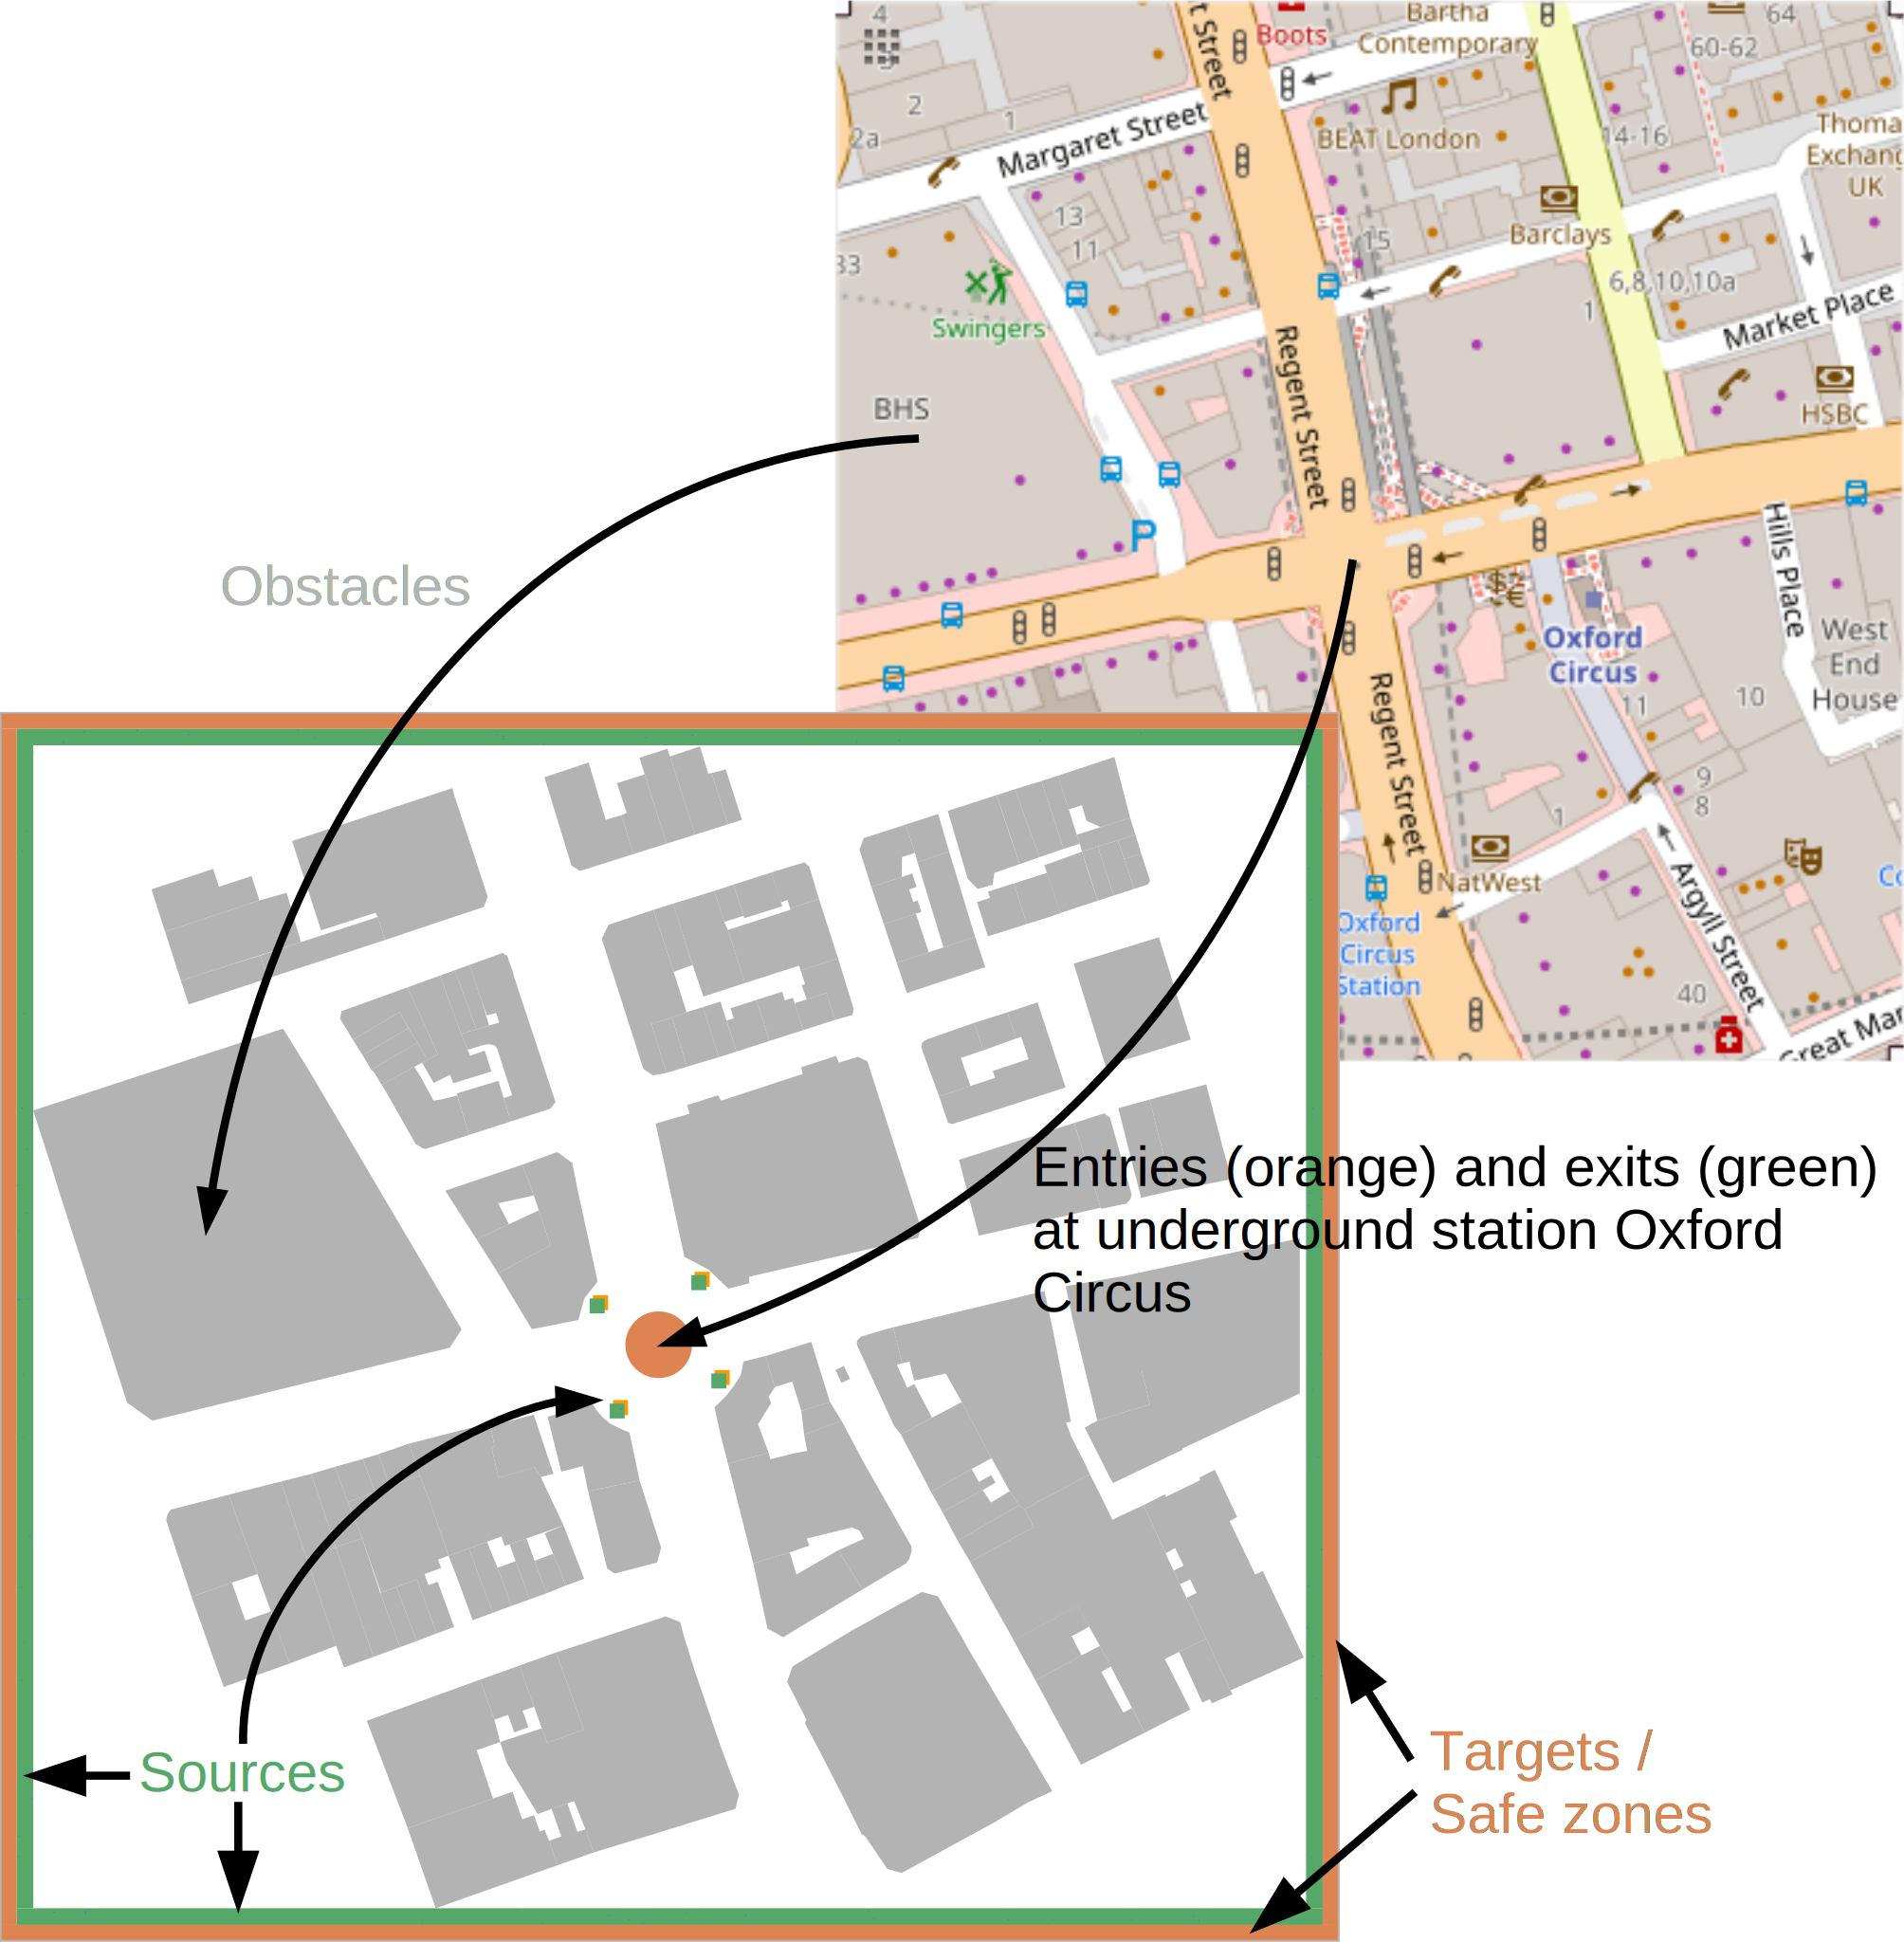
\includegraphics[width=\textwidth]{UseCasesAndValidation/SelfCatThreatModel/OpenStreetMap/SimulationArea-06}}
            \only<10>{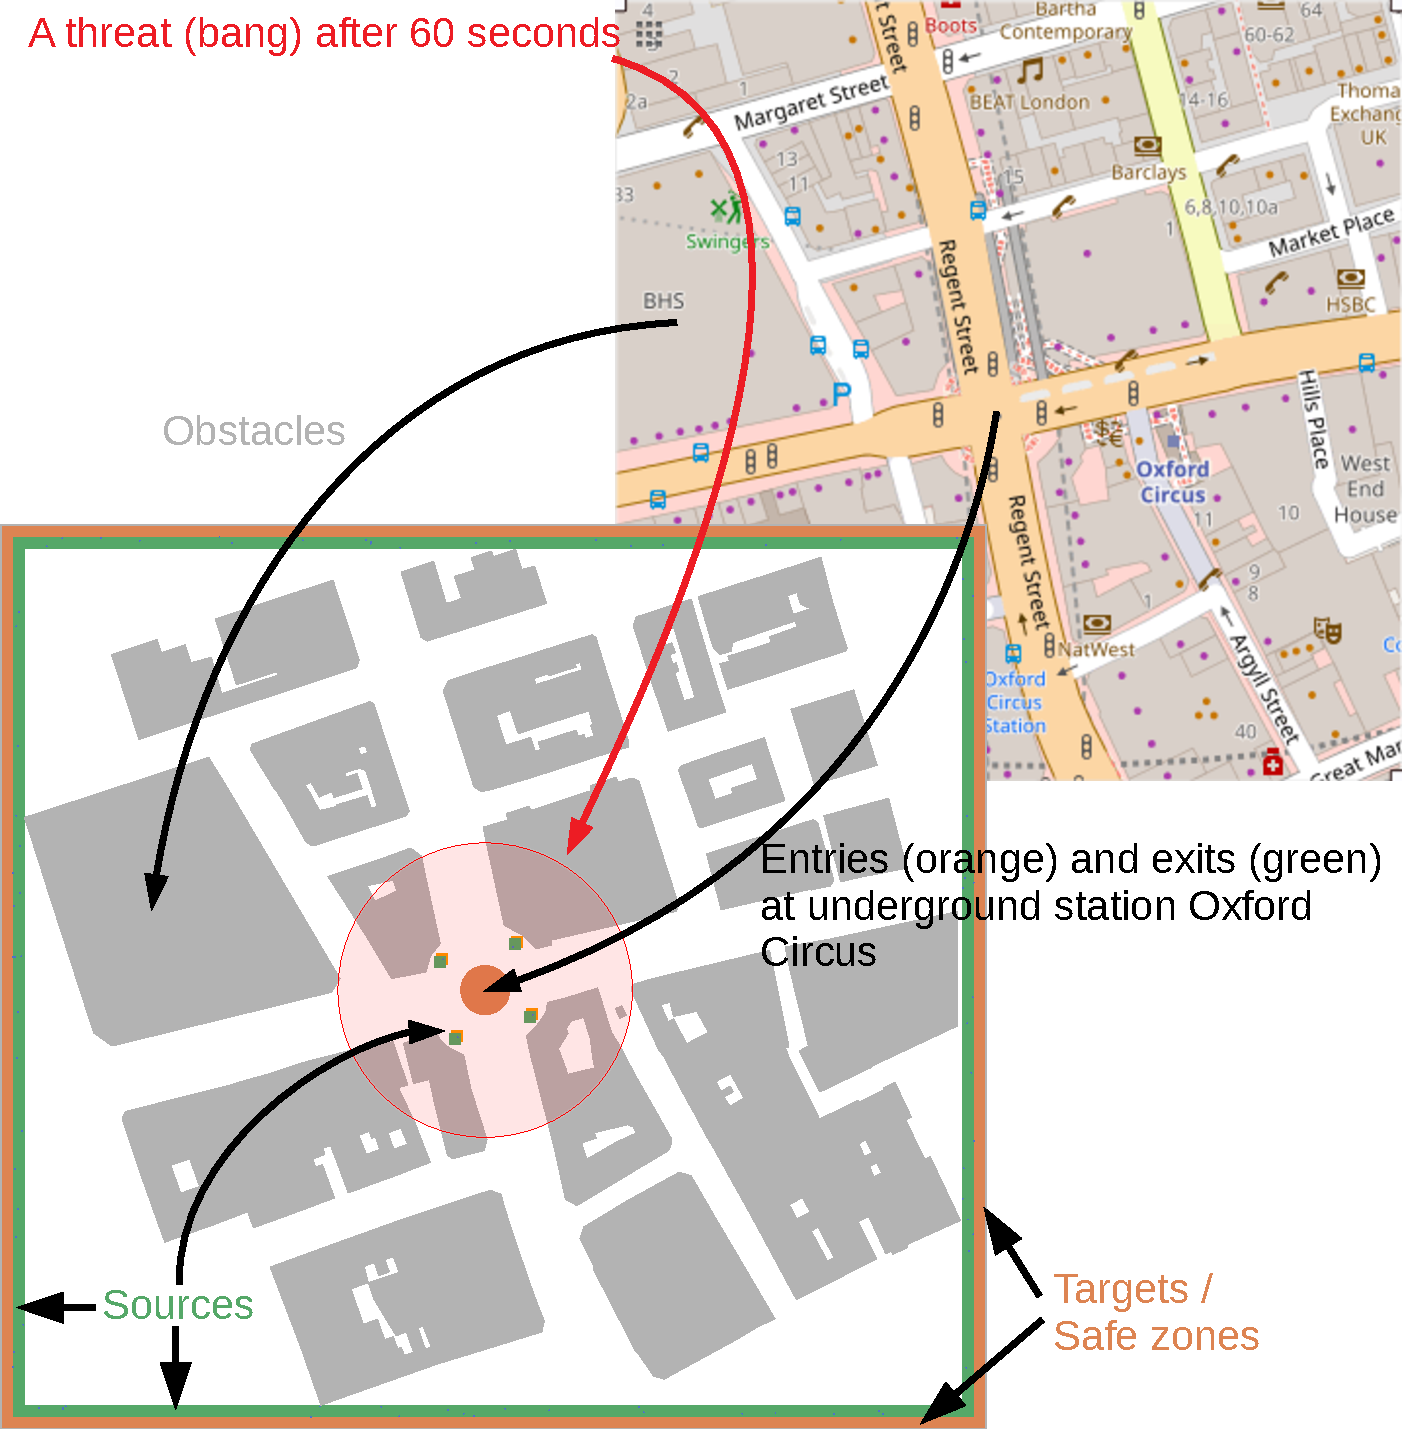
\includegraphics[width=\textwidth]{UseCasesAndValidation/SelfCatThreatModel/OpenStreetMap/SimulationArea-07}}
            \only<10>{\usebeamerfont{caption} \href{run:./Videos/Validation-UseCase2-SelfCatThreatModel.mp4}{\faPlayCircleO\ Simulation}}
        \end{minipage}
    \end{columns}
    
    \note<1>[item]{We could observe three different behaviors and a change between these behaviors.}
    \note<1>[item]{First, people were leaving an underground station very target-oriented.}
    \note<2>[item]{After, perceiving a loud bang --- an environmental stimulus --- the people were escaping.}
    \note<3>[item]{People, who did not perceive the bang, imitated other fleeing people.}
    \note<3>[item]{This is were social psychology comes into play and the evaluation of the local neighborhood is important and if agents feel in-group or out-group to each other. That is if they trust each other or not.}
    \note<4>[item]{I reenacted this simulation setup in the Vadere simulator in which I implemented the psychology layer.}
    \note<4>[item]{I imported the scene from OpenStreetMap so that buildings are represented as obstacles in the simulation.}
    \note<4>[item]{I placed sources for agents the leave the underground station and agents that head towards the station.}
    \note<4>[item]{And I placed a threat (a loud bang) at the underground station that causes agents to escape.}
    
\end{frame}


\begin{frame}{Perceived threat: Simulation results}
    \begin{columns}[T]
        \column{0.5\textwidth}
        \begin{minipage}[c][0.4\textheight][t]{\textwidth}
            \centering
            \only<1>{\includegraphics[width=\linewidth]{UseCasesAndValidation/SelfCatThreatModel/ParameterStudy/probabilityInGroupMembership/Boxplot-probabilityInGroupMembership-Range0to10}}
            \only<2>{\includegraphics[width=\linewidth]{UseCasesAndValidation/SelfCatThreatModel/ParameterStudy/probabilityInGroupMembership/Scatter-probabilityInGroupMembership-Range0to10}} % 30 runs per parameter set
        \end{minipage}
        \column{0.5\textwidth}
        \begin{minipage}[c][0.4\textheight][t]{\textwidth}
            \begin{itemize}
                \item Quantified: Decreasing evacuation time
                \item The reusable psychology layer is a benefit for practitioners.
                \item They can scrutinize \enquote{collective flight} incidents.
                \begin{itemize}
                    \pgfsetfillopacity{\myhide}
                    \item When and how do people flee?
                    \item When do they follow (or ignore) others?
                    \item ...
                \end{itemize}
            \end{itemize}
        \end{minipage}
    \end{columns}
    
    \note[item]{An interesting question arose: How is the evacuation time affected if people trust each other or not. That means how like is it that agents imitate the escaping behavior.}
    \note[item]{Simulations allowed us to test this without harming people and gives practitioners useful insights into crowd events and how to make them safer.}
\end{frame}

\begin{frame}{Modeling approaches: Pedestrian dynamics \hfill \hyperlink{BackupSlides}{\beamerbutton{Back}}}
\label{Backup:NavigationAndWayfinding}

    \small
    \only<1>{
        \begin{tabularx}{1.03\textwidth}{ | M{0.4\textwidth} M{0.55\textwidth}| }
            \hline
            \textbf{Macroscopic} &  \\[-2mm]
            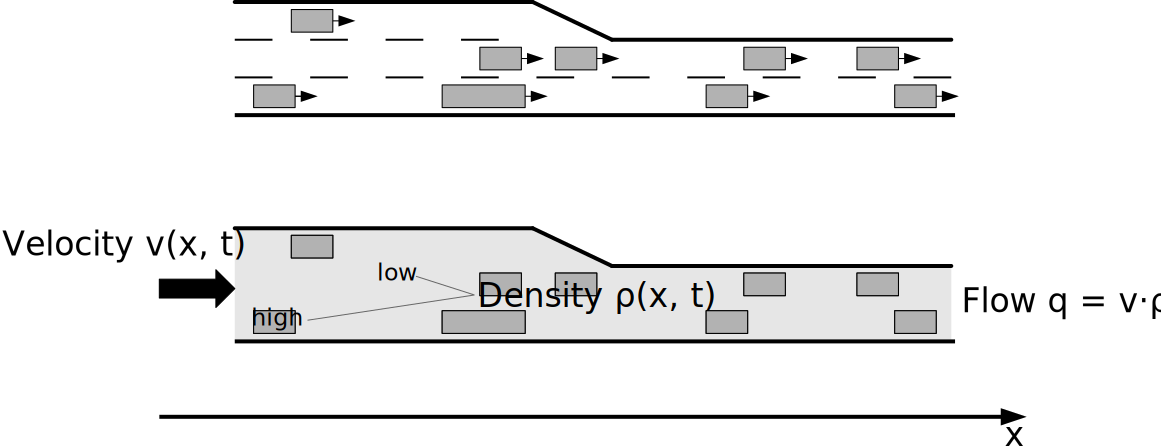
\includegraphics[height=1.8cm]{PedestrianStreamSimulations/Macroscopic/MacroscopicModels-LiquidizationTrafficFlow} & \begin{itemizetab}
                \item Individuals are seen as continuum
                \item Usually, expressed as differential equations, i.e. density or concentration evolution over time
            \end{itemizetab} \\[-3mm]
            \hline
            \textbf{Mesoscopic (multi-scale)} &  \\[-2mm]
            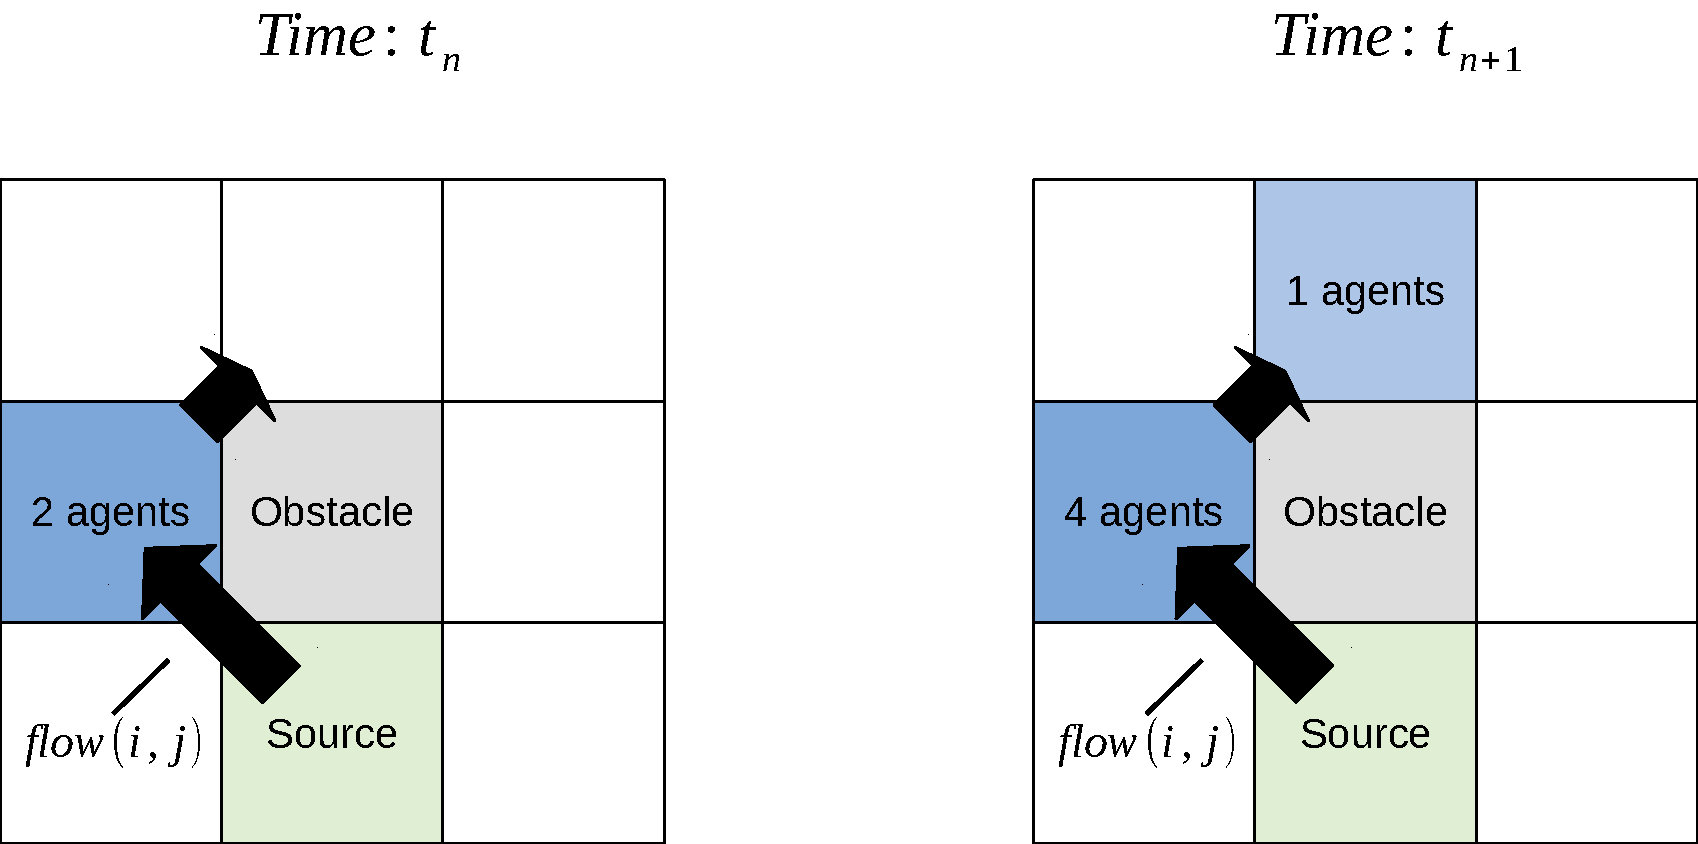
\includegraphics[height=1.8cm]{PedestrianStreamSimulations/Mesoscopic/LocomotionModels-Mesoscopic-CellMovement-RectangularFlow} & \begin{itemizetab}
                \item Simulation area is divided into cells where one cell can contain multiple agents
                \item Flow between cells is modeled based on properties of individuals
            \end{itemizetab} \\[-3mm]
            \hline
            \textbf{Microscopic} &  \\[-2mm]
            \includegraphics[height=1.8cm]{PedestrianStreamSimulations/Microscopic/ModelingCompontentsFromKleinmeier2019/BasicComponents} & \begin{itemizetab}
                \item Each agent has several attributes, e.g. preferred speed etc.
                \item The agent motion is modeled for each agent individually
            \end{itemizetab} \\
            \hline
        \end{tabularx}
    }
    \only<2>{
        \begin{tabularx}{1.03\textwidth}{ | M{0.4\textwidth} M{0.55\textwidth}| }
            \hline
            \textbf{Macroscopic} &  \\[-2mm]
            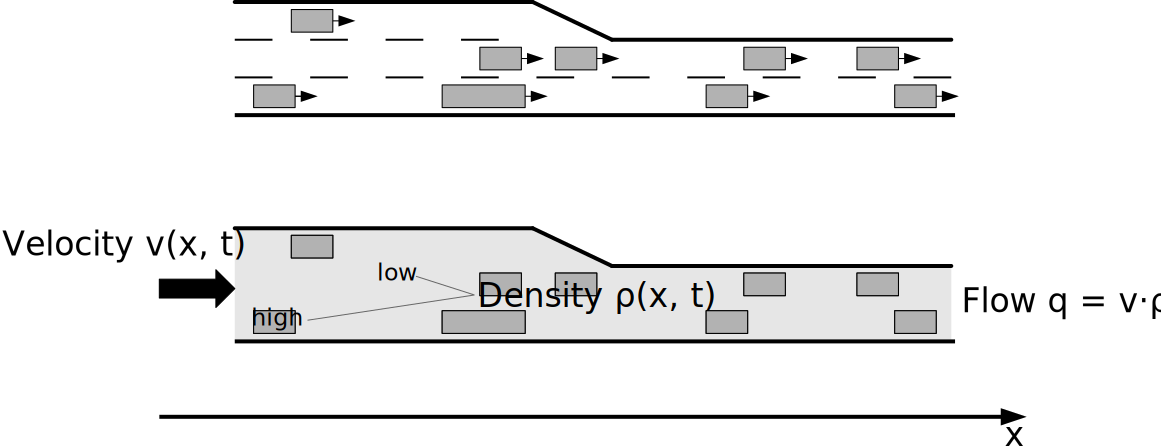
\includegraphics[height=1.8cm]{PedestrianStreamSimulations/Macroscopic/MacroscopicModels-LiquidizationTrafficFlow} & \begin{itemizetab}
                \item Individuals are seen as continuum
                \item Usually, expressed as differential equations, i.e. density or concentration evolution over time
            \end{itemizetab} \\[-3mm]
            \hline
            \textbf{Mesoscopic (multi-scale)} &  \\[-2mm]
            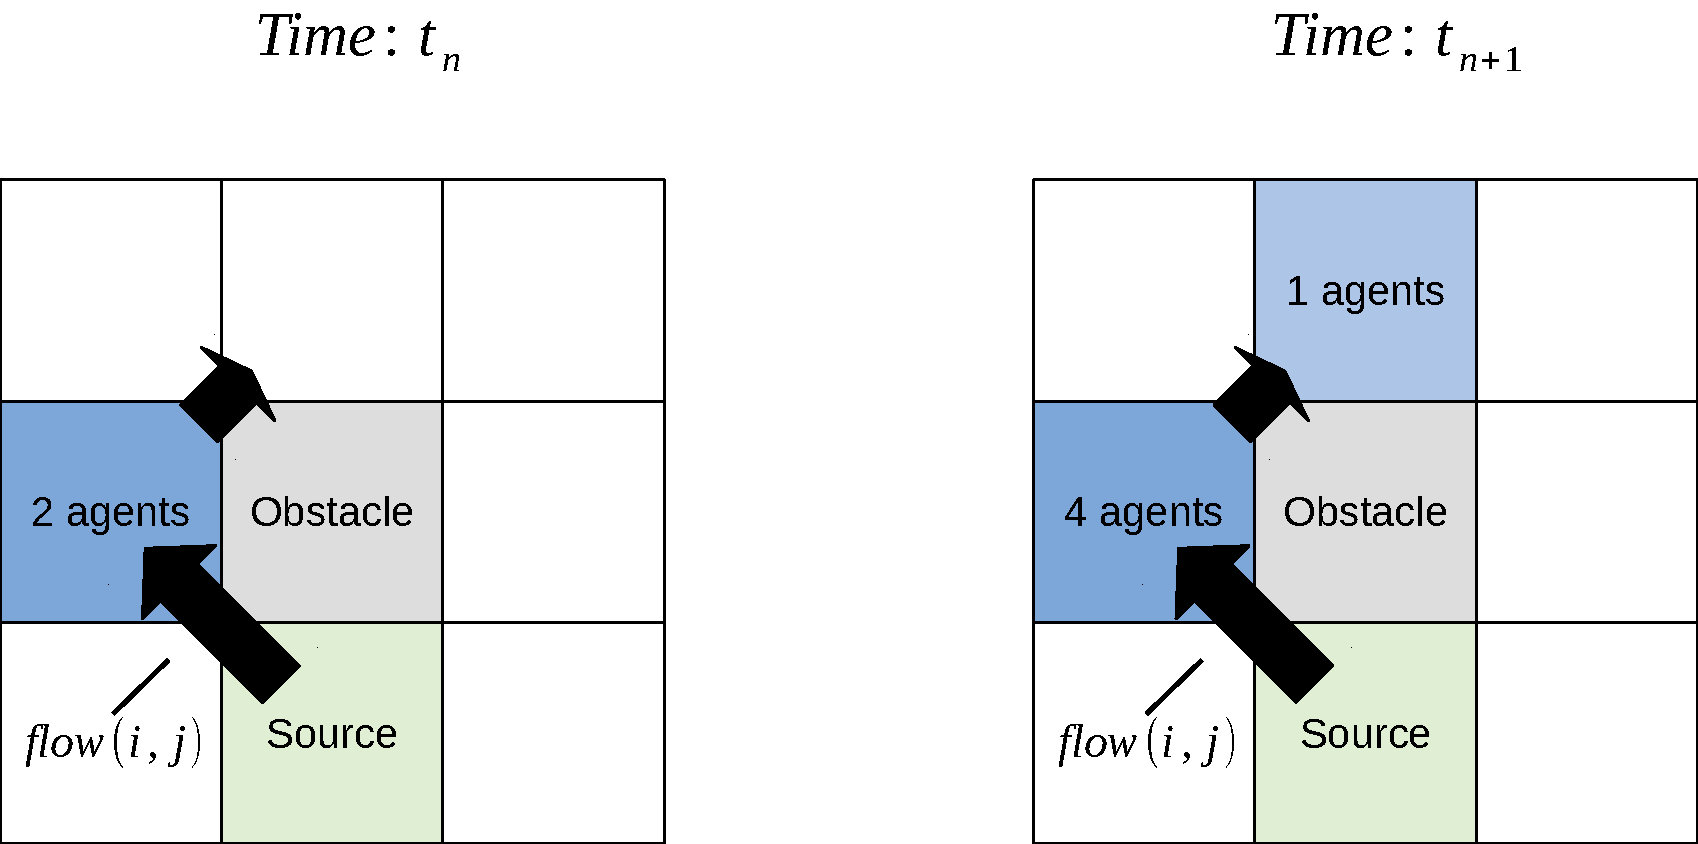
\includegraphics[height=1.8cm]{PedestrianStreamSimulations/Mesoscopic/LocomotionModels-Mesoscopic-CellMovement-RectangularFlow} & \begin{itemizetab}
                \item Simulation area is divided into cells where one cell can contain multiple agents
                \item Flow between cells is modeled based on properties of individuals
            \end{itemizetab} \\[-3mm]
            \hline
            \textbf{Microscopic} &  \\[-2mm]
            \includegraphics[height=1.8cm]{PedestrianStreamSimulations/Microscopic/LocomotionModels/CellularAutomata-Grid} & \begin{itemizetab}
                \item Each agent has several attributes, e.g. preferred speed etc.
                \item The agent motion is modeled for each agent individually
            \end{itemizetab} \\
            \hline
        \end{tabularx}
    }
    
    \note<1>[item]{First it is important to know existing approaches how pedestrian streams and crowds have been modeled so far.}
    \note<1>[item]{These approaches can be reused and must not be reinvented because they work already pretty well as we have seen in the video.}
    \note<1>[item]{These approaches can be divided into macroscopic, microscopic and mesoscopic, also called multi-scale, models which combine macroscopic and microscopic approaches.}
    \note<1>[item]{In macroscopic models, individuals are see as continuum, for example as density.}
    \note<1>[item]{Then, this density evolution is expressed as differential equation.}
    \note<1>[item]{\todo{Mention drawback}}
    
    \note<2>[item]{Another approach is to divide the simulation area into cells where one cell can be occupied by multiple agents.}
    \note<2>[item]{Then, the flow between these cells is modeled.}
    \note<2>[item]{\todo{Mention drawback}}
    
    \note<2>[item]{In microscopic models, individual agents are moved in the simulation area by using different techniques.}
    \note<2>[item]{\todo{Describe micro model and the central aspect of navigation and wayfinding algorithms. A modern approach is to use the eikonal equation, an equation which describes a propagating wave. Each wave front represents the travel time to the wave origin.}}
    \note<2>[item]{In my implementation, I reused existing microscopic locomotion techniques.}
\end{frame}

\begin{frame}[allowframebreaks]{References}
    \nocite{sivers-2015c,kleinmeier-2019,zoennchen-2019b,kleinmeier-2019b,kleinmeier-2020}
    
    \renewcommand*{\bibfont}{\tiny}
    \printbibliography
\end{frame}

\end{document}
